%!TEX root=../../main.tex

\section{Backend und Infrastruktur}
\subsection{Einleitung}
Der Anspruch an die Infrastruktur und an das Backend besteht darin, die Software als ganzes zu steuern und zu erhalten. Die Infrastruktur muss einfach zu aufbauen und zu starten sein. Die folgenden Kapiteln erläutern nach der generellen Analyse von Lösungsmöglichkeiten im \autoref{chap:backendsota} nun einen ausgearbeiteten Plan, wie die später folgende Implementierung aussehen soll. Hierfür werden Graphiken oder Tabelle verwendet. Sie sollen ausreichend Informationen über Abläufe oder verschiedene Funktionalität vorgeben, um diese entsprechend daraufhin zu implementieren. Des Weiteren sollen die genormten Diagrammarten dazu dienen das komplexe Backend und die Infrastruktur einfach und übersichtlich darzustellen, um speziell die Schnittstellenherausforderungen verständlich zu machen.
\subsection{Infrastruktur}
Die Infrastruktur enthält jegliche Dienste und Anwendungen, welche von der Software in der Projektumgebung benötigt werden. Um diese Dienste mit einfach aufbauen zu können wird eine Virtualisierung über Container mittels Docker umgesetzt. Diese virtuellen Instanzen verbunden in einem Docker-Compose Stack werden über ein eigenes Skript gesteuert.
\subsubsection{Docker Stack}
\begin{figure}[H]
	\centering
	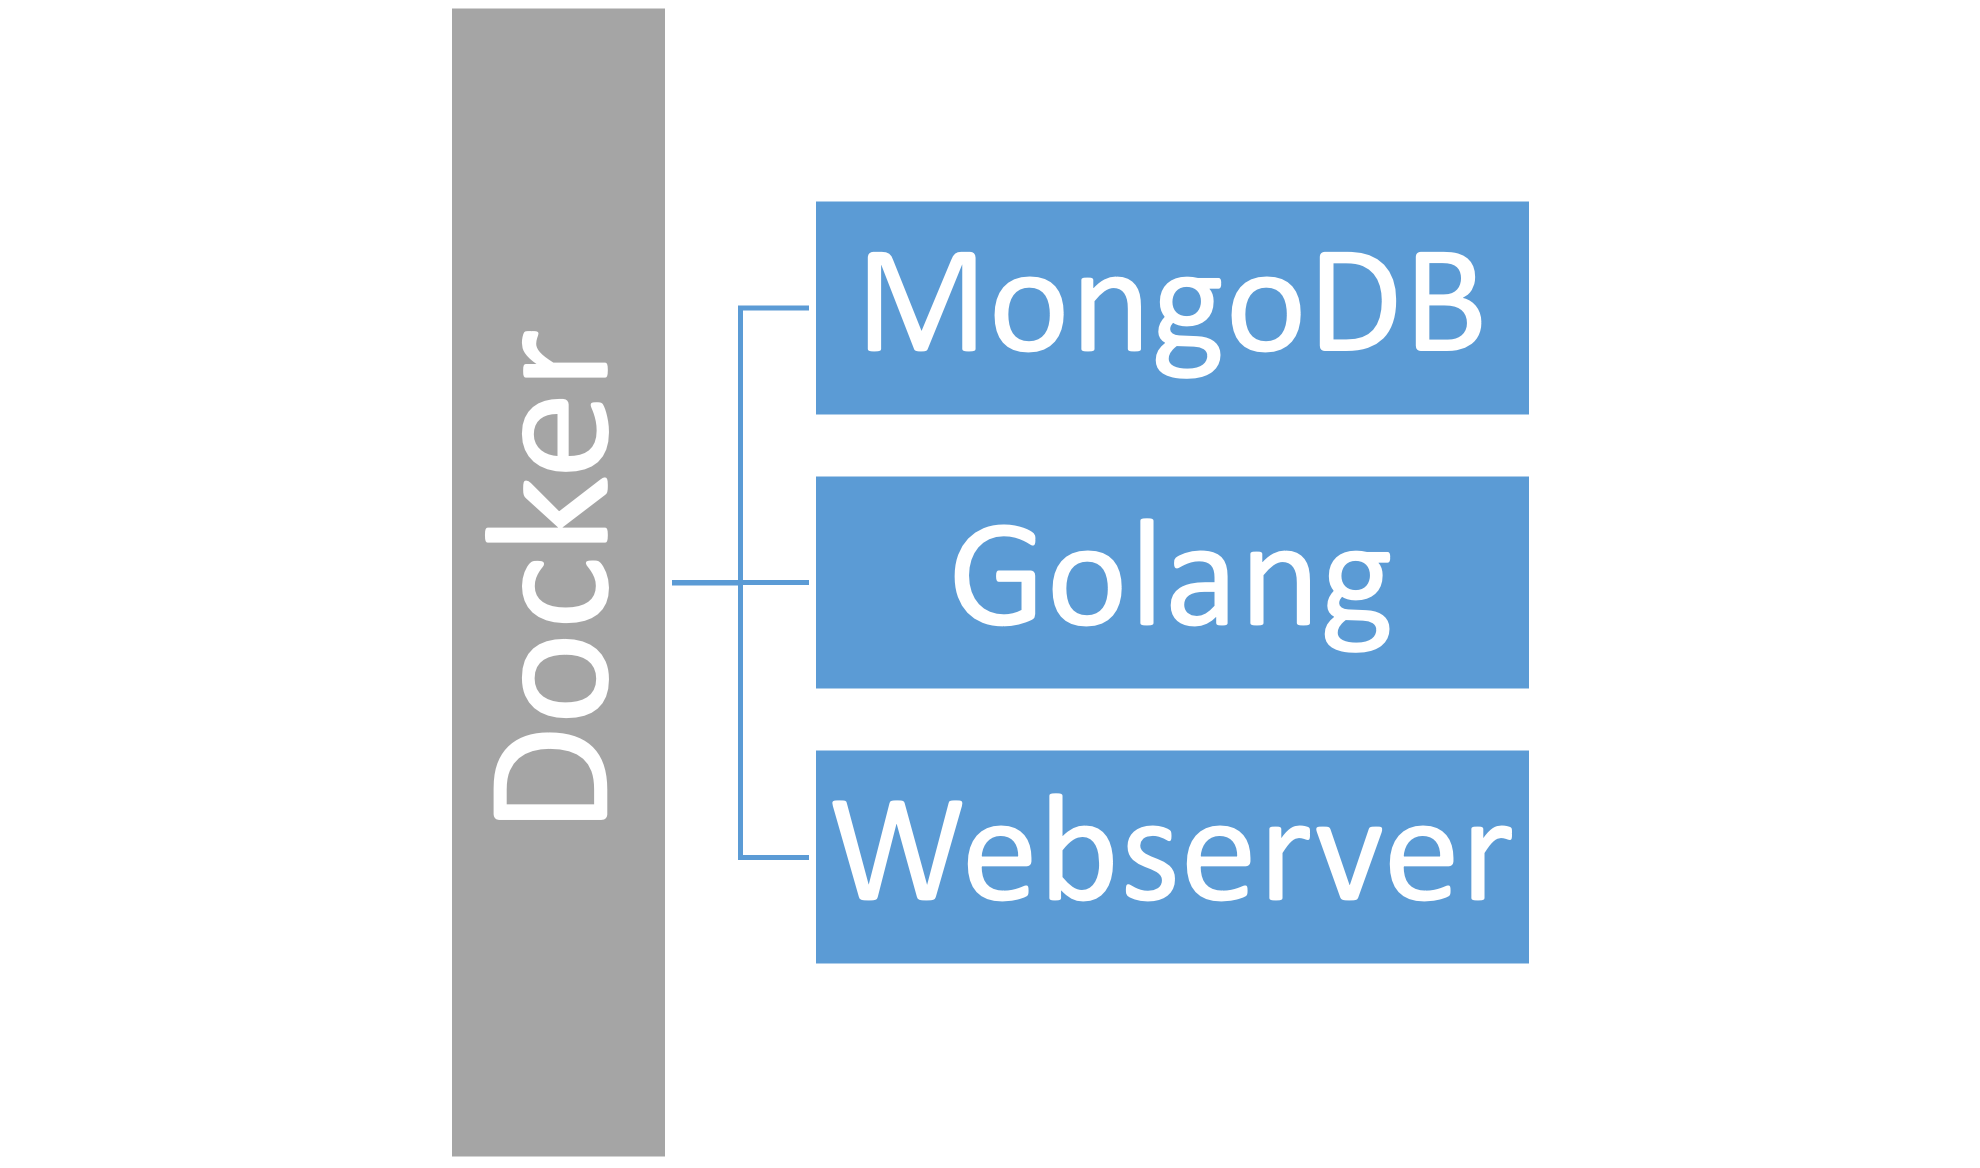
\includegraphics[width=\linewidth]{images/mbeier_konzept/docker-stack}
	\caption[Docker-Compose Stack]{Übersicht über die Container des Docker-Compose Stack}
	\label{fig:docker-stack}
\end{figure}

\newpage

Diese in Docker Container befindlichen Dienste und Anwendungen werden benötigt um die Software funktionsfähig bereitzustellen. Der automatische Aufbau dieser Container-Infrastruktur geschieht auf Basis einer Docker-Compose Konfiguration automatisch. \\

Docker Container stellen eigene Umgebungen dar, welche nach dem stoppen oftmals vollständig zerstört und gelöscht werden. Die Daten, auf die die Software und auch die anderen Anwendungen zugreifen müssen, sind jedoch über die Lebenszeit eines Docker Container darüber hinaus zu persistieren. Um dies garantieren zu können, werden Volumes in die Container eingehängt, so dass die Daten prinzipiell außerhalb der Container gespeichert wird und nur von außen in die Umgebungen eingehängt werden. Dies ist bei dem MongoDB Container erforderlich, um die Daten, welche in der Datenbank gespeichert werden, permanent zu speichern. Ebenso ist es erforderlich die generierten Dateien des Golang-Backends zu persistieren, um auf diese später wieder zugreifen zu können. Auch werden im Backend diverse gleichbleibende Passphrasen, beispielsweise zum Signieren von Tokens, auf die gleiche Art und Weise gespeichert. \\

Die Zugangsdaten für den Nutzeraccount, welche beim Installieren abgefragt werden (siehe \autoref{fig:install}), der Datenbank werden über Dockers Secrets-Management sowohl in den Datenbank-, als auch in den Golang-Container, damit sich dieser zur Datenbank verbinden kann, eingehängt. In der Datenbank müssen initial neben den Datenbanknutzern auch die Datenbankinstanz selbst angelegt werden. Dies geschieht über ein eigenes zum Start ausführendes Skript. \\

Das Frontend selbst besteht aus zwei Ebenen. Zu Beginn am Start wird das Frontend selbst kompiliert und installiert. Hierfür gibt es einen eigenen Container, der hierfür eine Umgebung bietet. Danach wird der eigentliche Webserver-Container gestartet und die zuvor kompilierten Dateien werden in den neuen Container kopiert. Ebenfalls wird eine angelegte Konfigurationsdatei, die den Webserver Dienst weitergehend konfiguriert, in das entsprechende Verzeichnis hinzugefügt.\\

% ToDo HTTPS Certificates

\newpage

\subsubsection{Steuerungsskript}

Das Steuerungsskript ermöglicht die genaue und einfache Steuerung der Infrastruktur.
Hierfür implementiert das Steuerungsskript folgende Submethoden mit entsprechenden Abläufen und Funktionalität:\\

\textbf{Installationsvorgang:}

\begin{figure}[H]
	\centering
	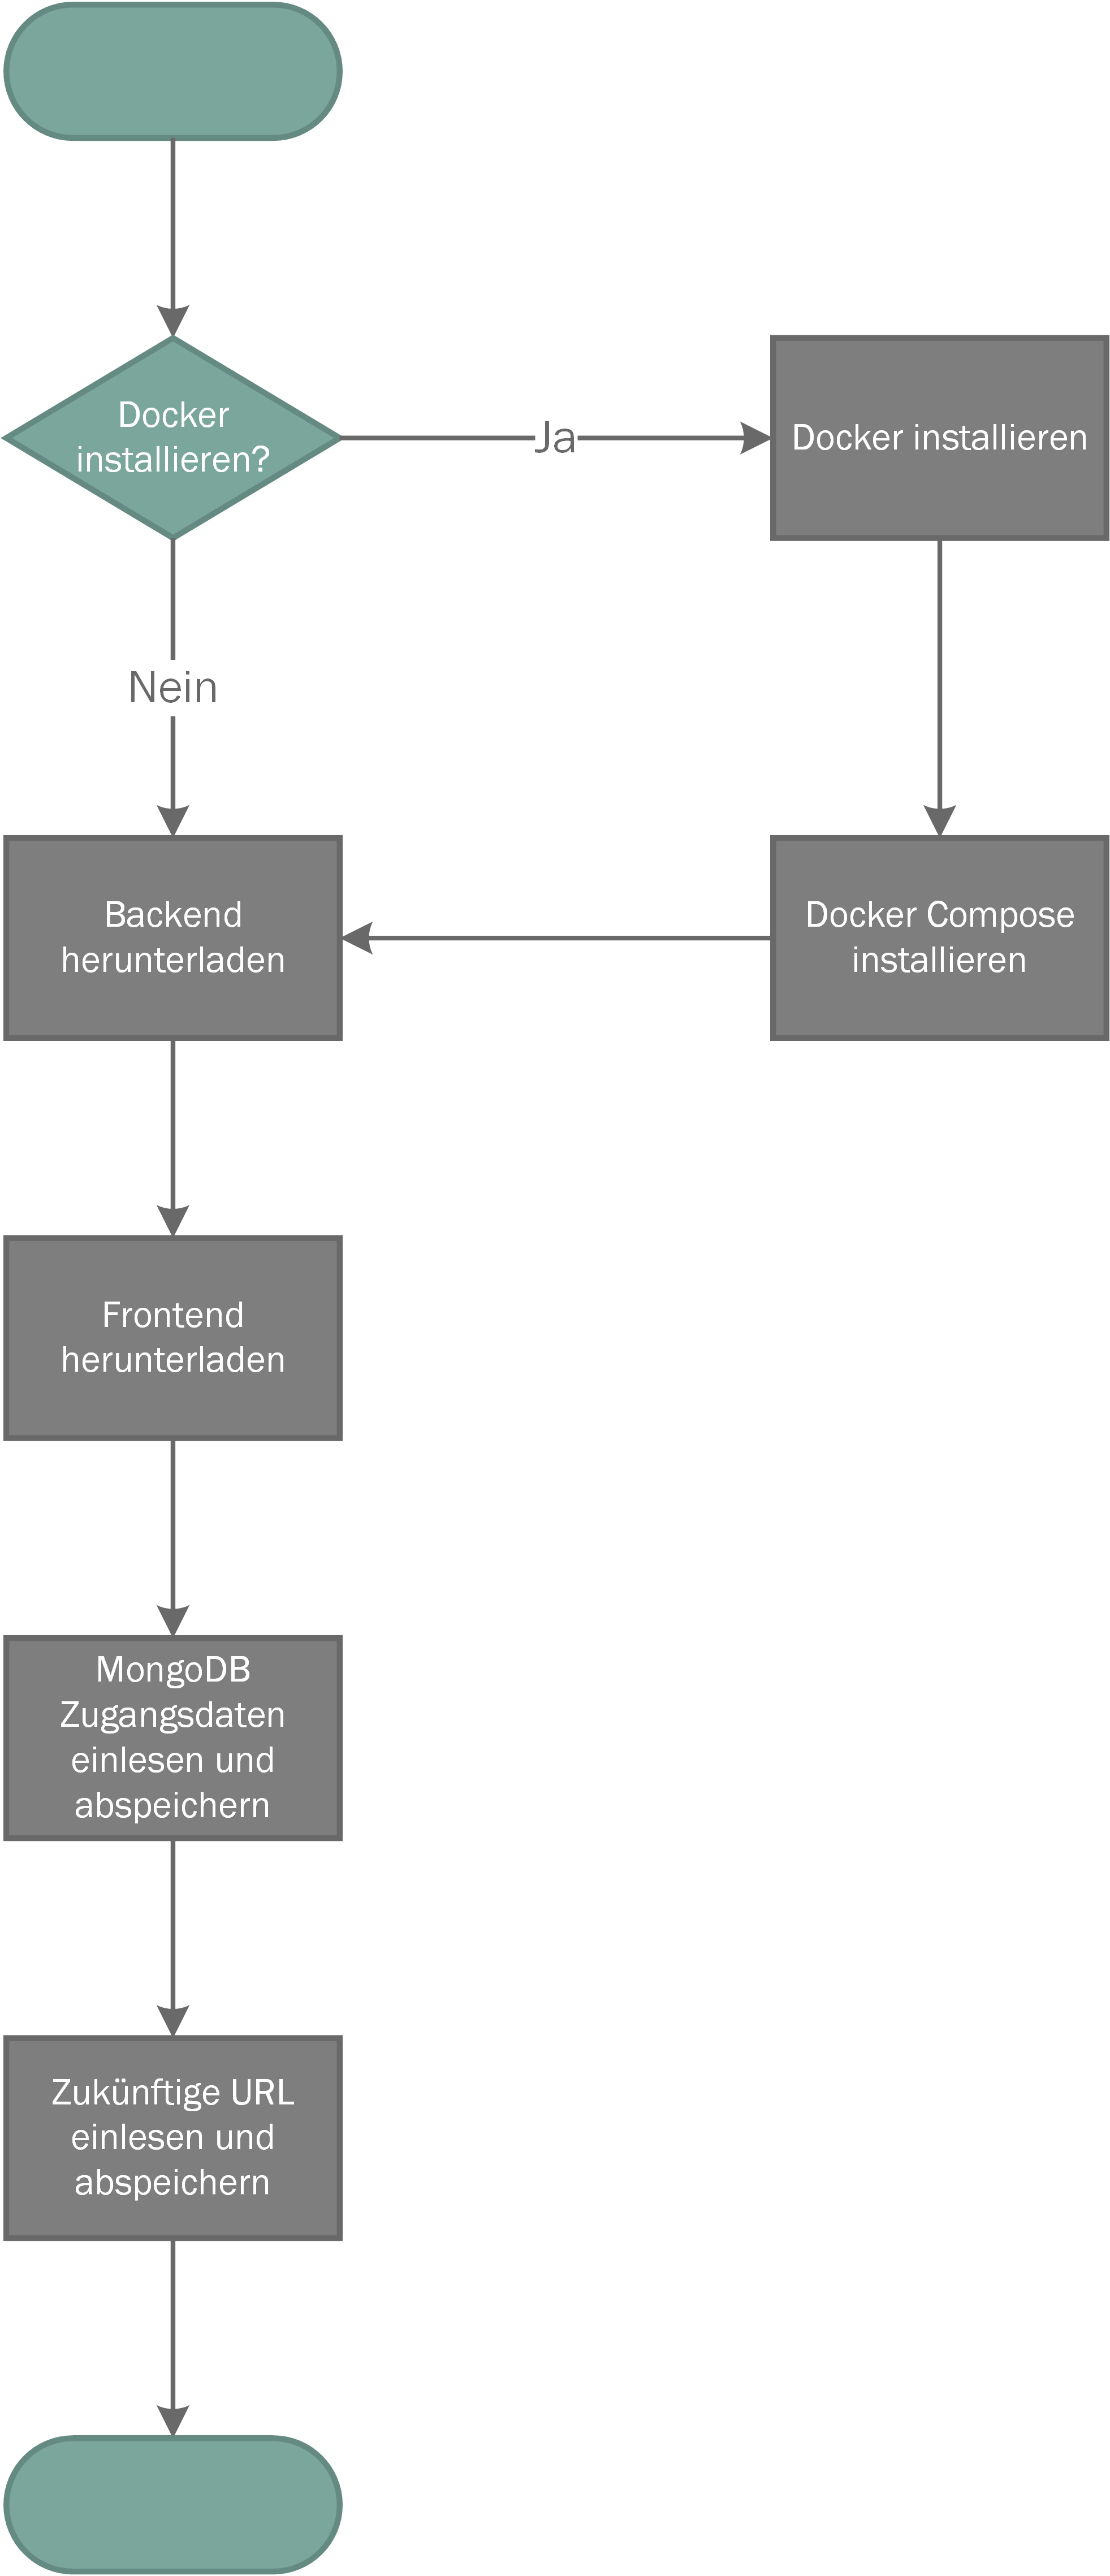
\includegraphics[width=0.5\linewidth]{images/mbeier_konzept/Install}
	\caption[Flussdiagramm über den Installationsvorgang]{Flussdiagramm über den Installationsvorgang}
	\label{fig:install}
\end{figure}

\newpage

Die Idee hinter der Etablierung eines Installationsvorganges soll die Einfachheit der Steuerung der Software hervorheben. Das Install-Repository beinhaltet hierbei lediglich eine grundlegende Ordnerstruktur und das Steuerungsskript selbst. Durch den Installationsvorgang werden die restlichen benötigten Daten automatisch heruntergeladen und installiert.

~\\~\\~\\
\textbf{Startvorgang:}

\begin{figure}[H]
	\centering
	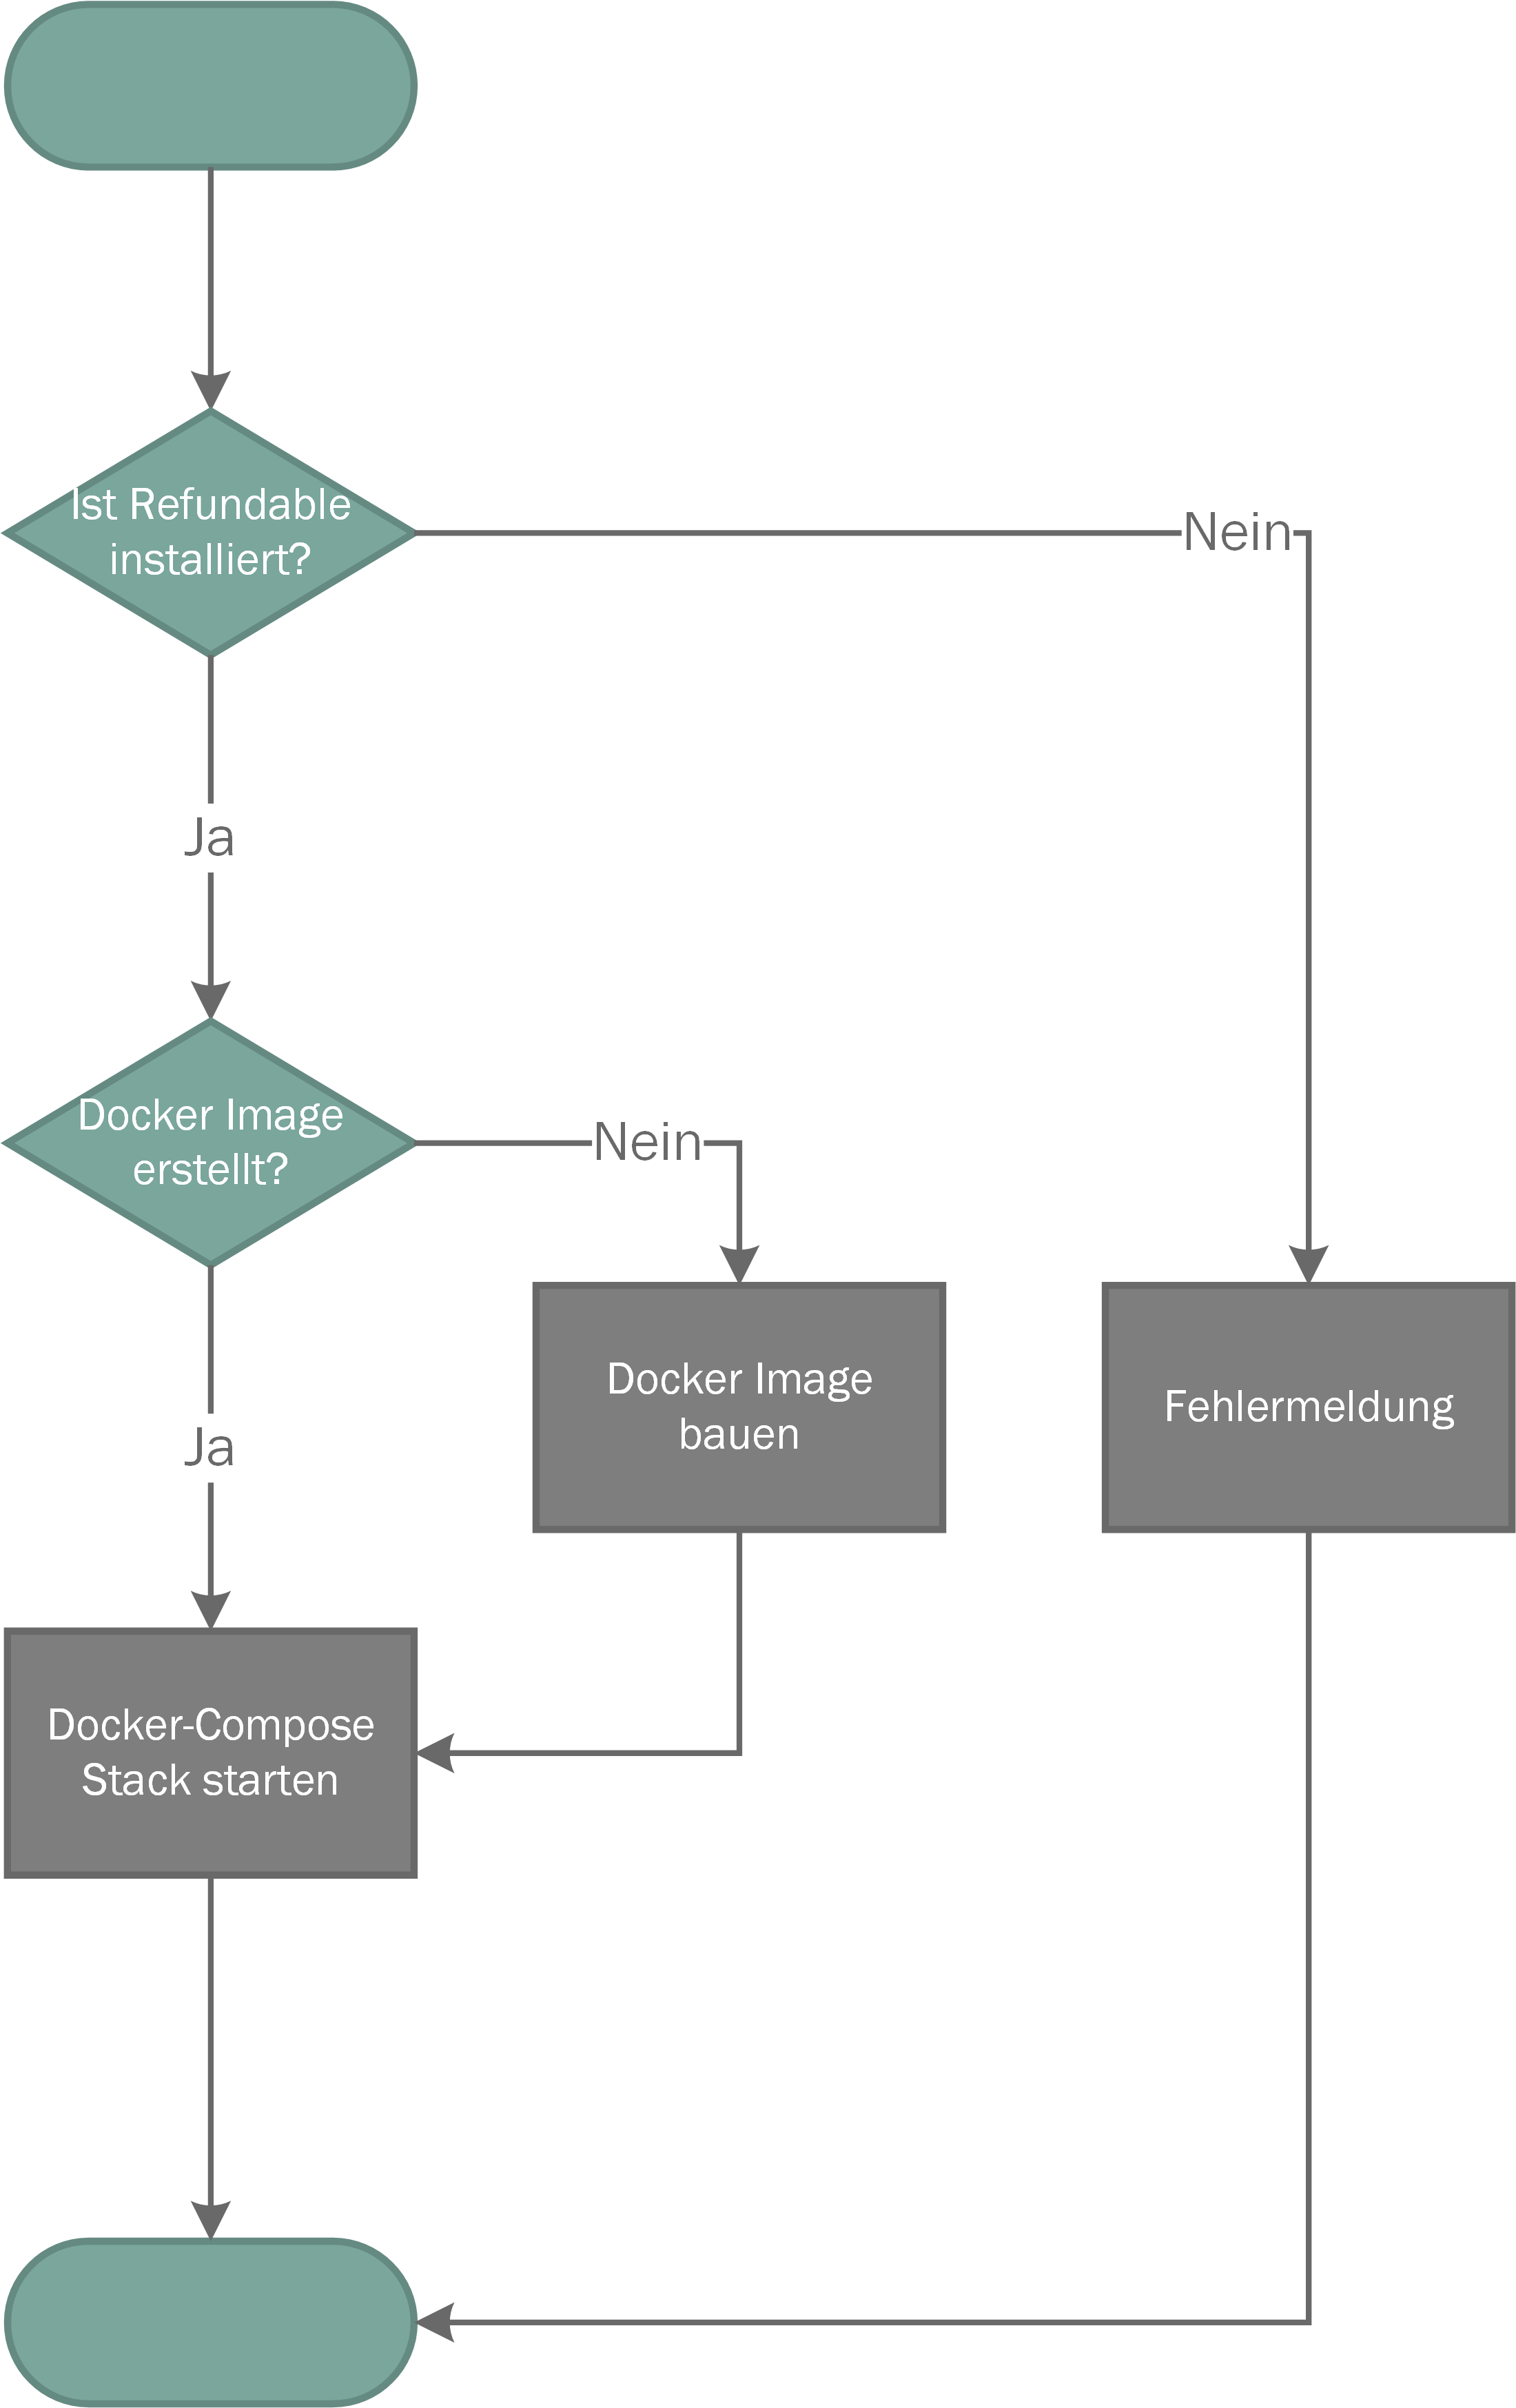
\includegraphics[width=0.5\linewidth]{images/mbeier_konzept/Start}
	\caption[Flussdiagramm über den Startvorgang]{Flussdiagramm über den Startvorgang}
	\label{fig:start}
\end{figure}

Der Startvorgang baut die Docker-Images, sofern diese noch nicht vorhanden sind, grundlegend auf Basis der installierten Dateien auf und startet daraufhin den gesamten Stack auf einmal. Voraussetzung hierfür ist, dass der Installationsvorgang bereits abgeschlossen ist und die heruntergeladenen Dateien vorhanden sind.

\newpage  

\textbf{Stoppvorgang:}

\begin{figure}[H]
	\centering
	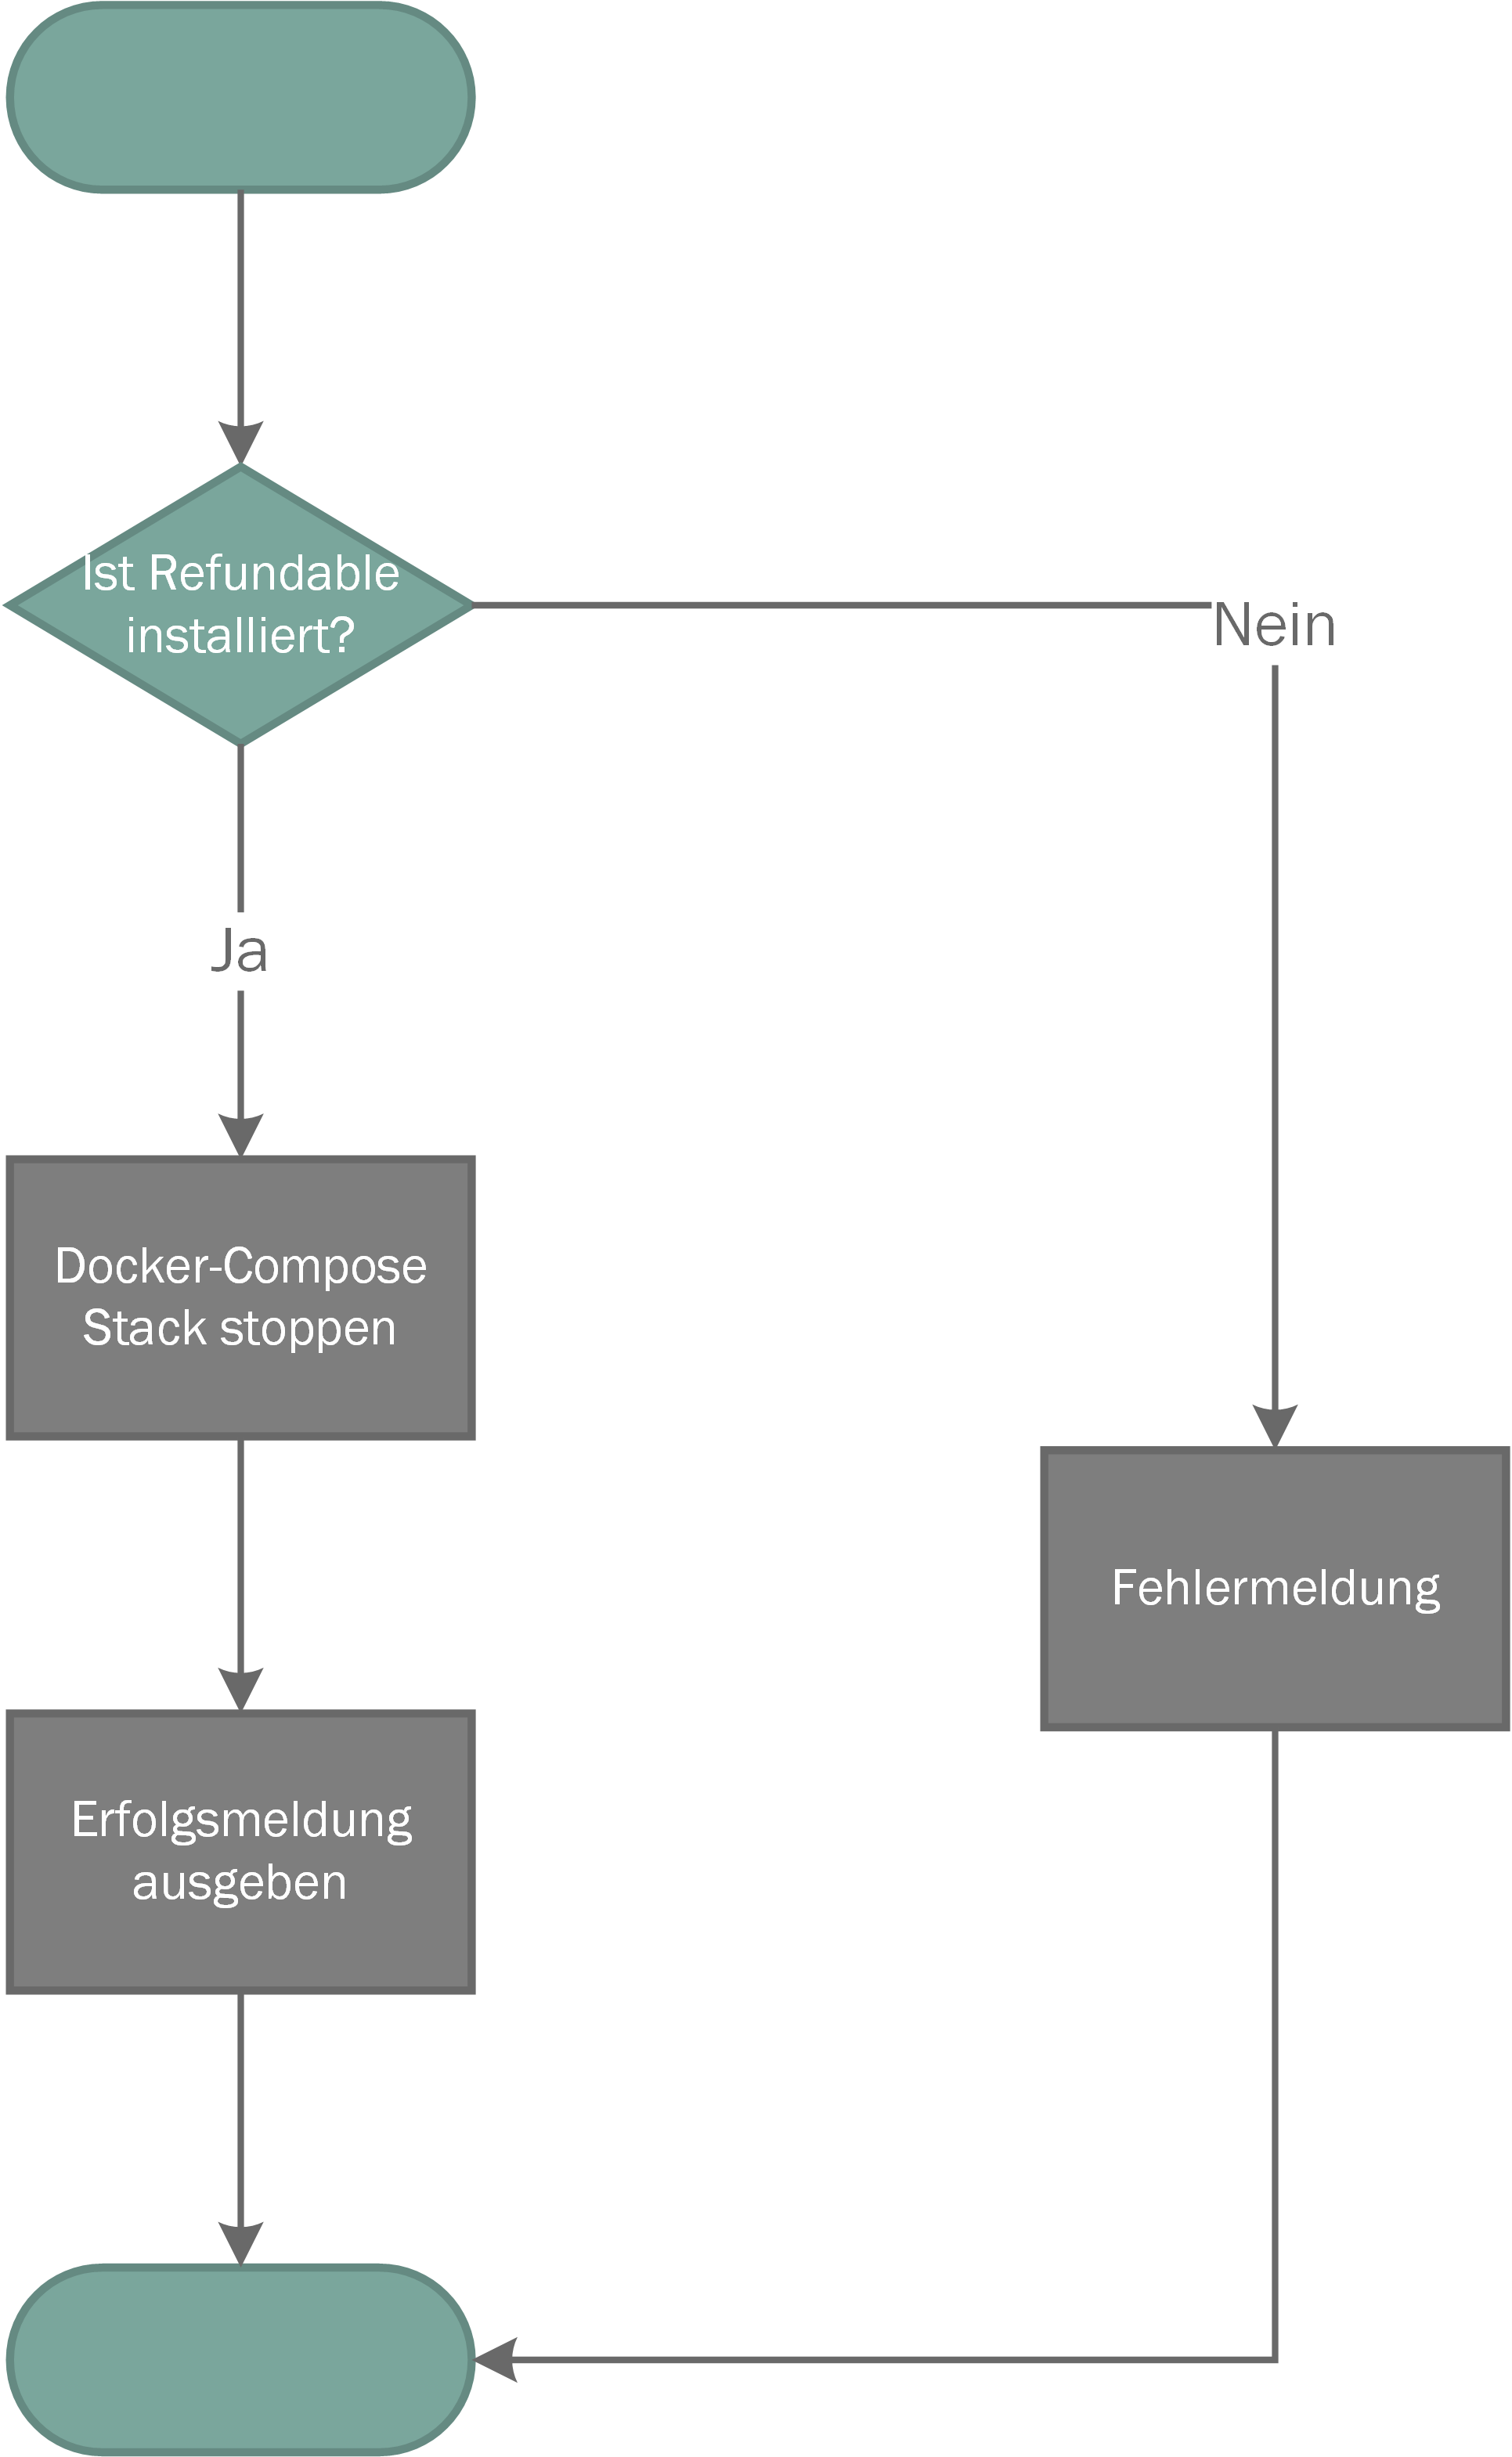
\includegraphics[width=0.5\linewidth]{images/mbeier_konzept/Stop}
	\caption[Flussdiagramm über den Stoppvorgang]{Flussdiagramm über den Stoppvorgang}
	\label{fig:stop}
\end{figure}

~\\
Der Stoppvorgang stoppt die laufenden Docker-Container und entfernt diese aus der Docker Umgebung. Dies führt dazu, dass garantiert wird, dass sich die wieder neu aufbauende Umgebung tatsächlich neu ist, und nicht nur eine alte Instanz wiederverwendet wird.

\newpage

\textbf{Neustartvorgang:}

\begin{figure}[H]
	\centering
	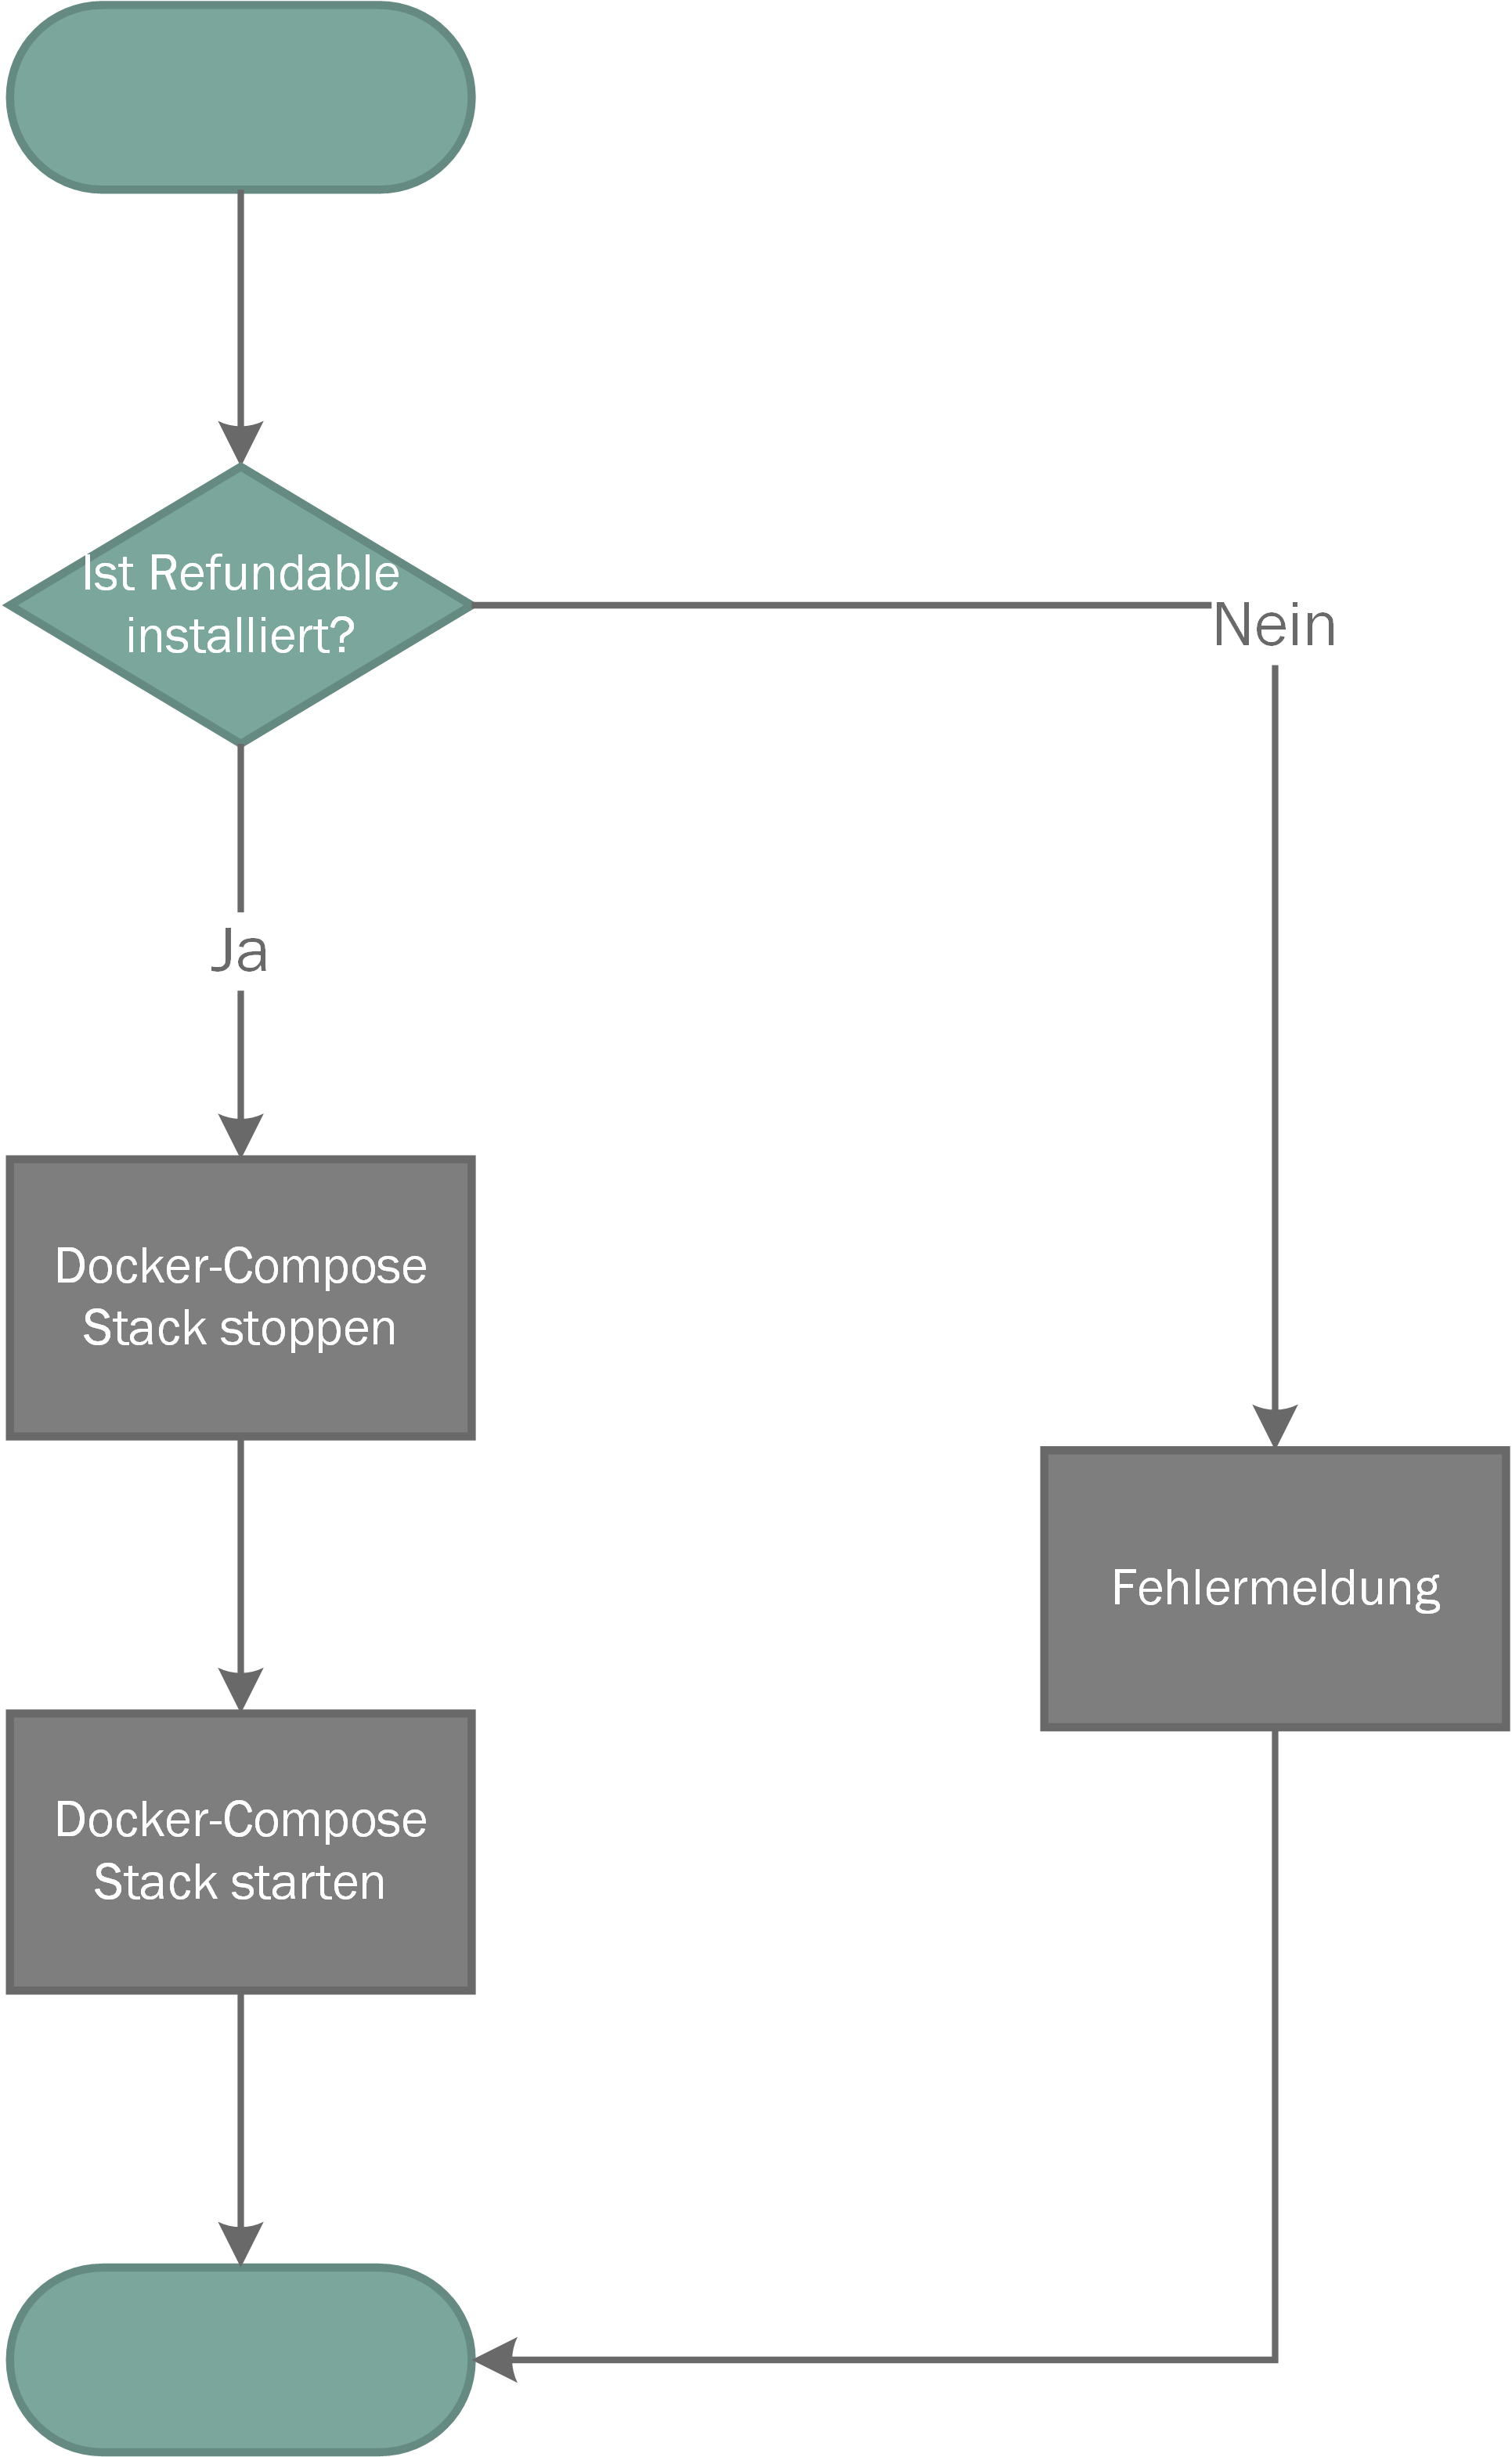
\includegraphics[width=0.5\linewidth]{images/mbeier_konzept/Restart}
	\caption[Flussdiagramm über den Neustartvorgang]{Flussdiagramm über den Neustartvorgang}
	\label{fig:restart}
\end{figure}
~\\
Der Neustartvorgang kombiniert den Start- und Stoppvorgang und führt diese beiden auf einmal aus. Er wird hauptsächlich dafür genutzt, um neue Konfigurationen, welche nur beim Start des Systems eingelesen werden, von der Software übernehmen zu lassen.

\newpage

\textbf{Aktualisierungsvorgang:}

\begin{figure}[H]
	\centering
	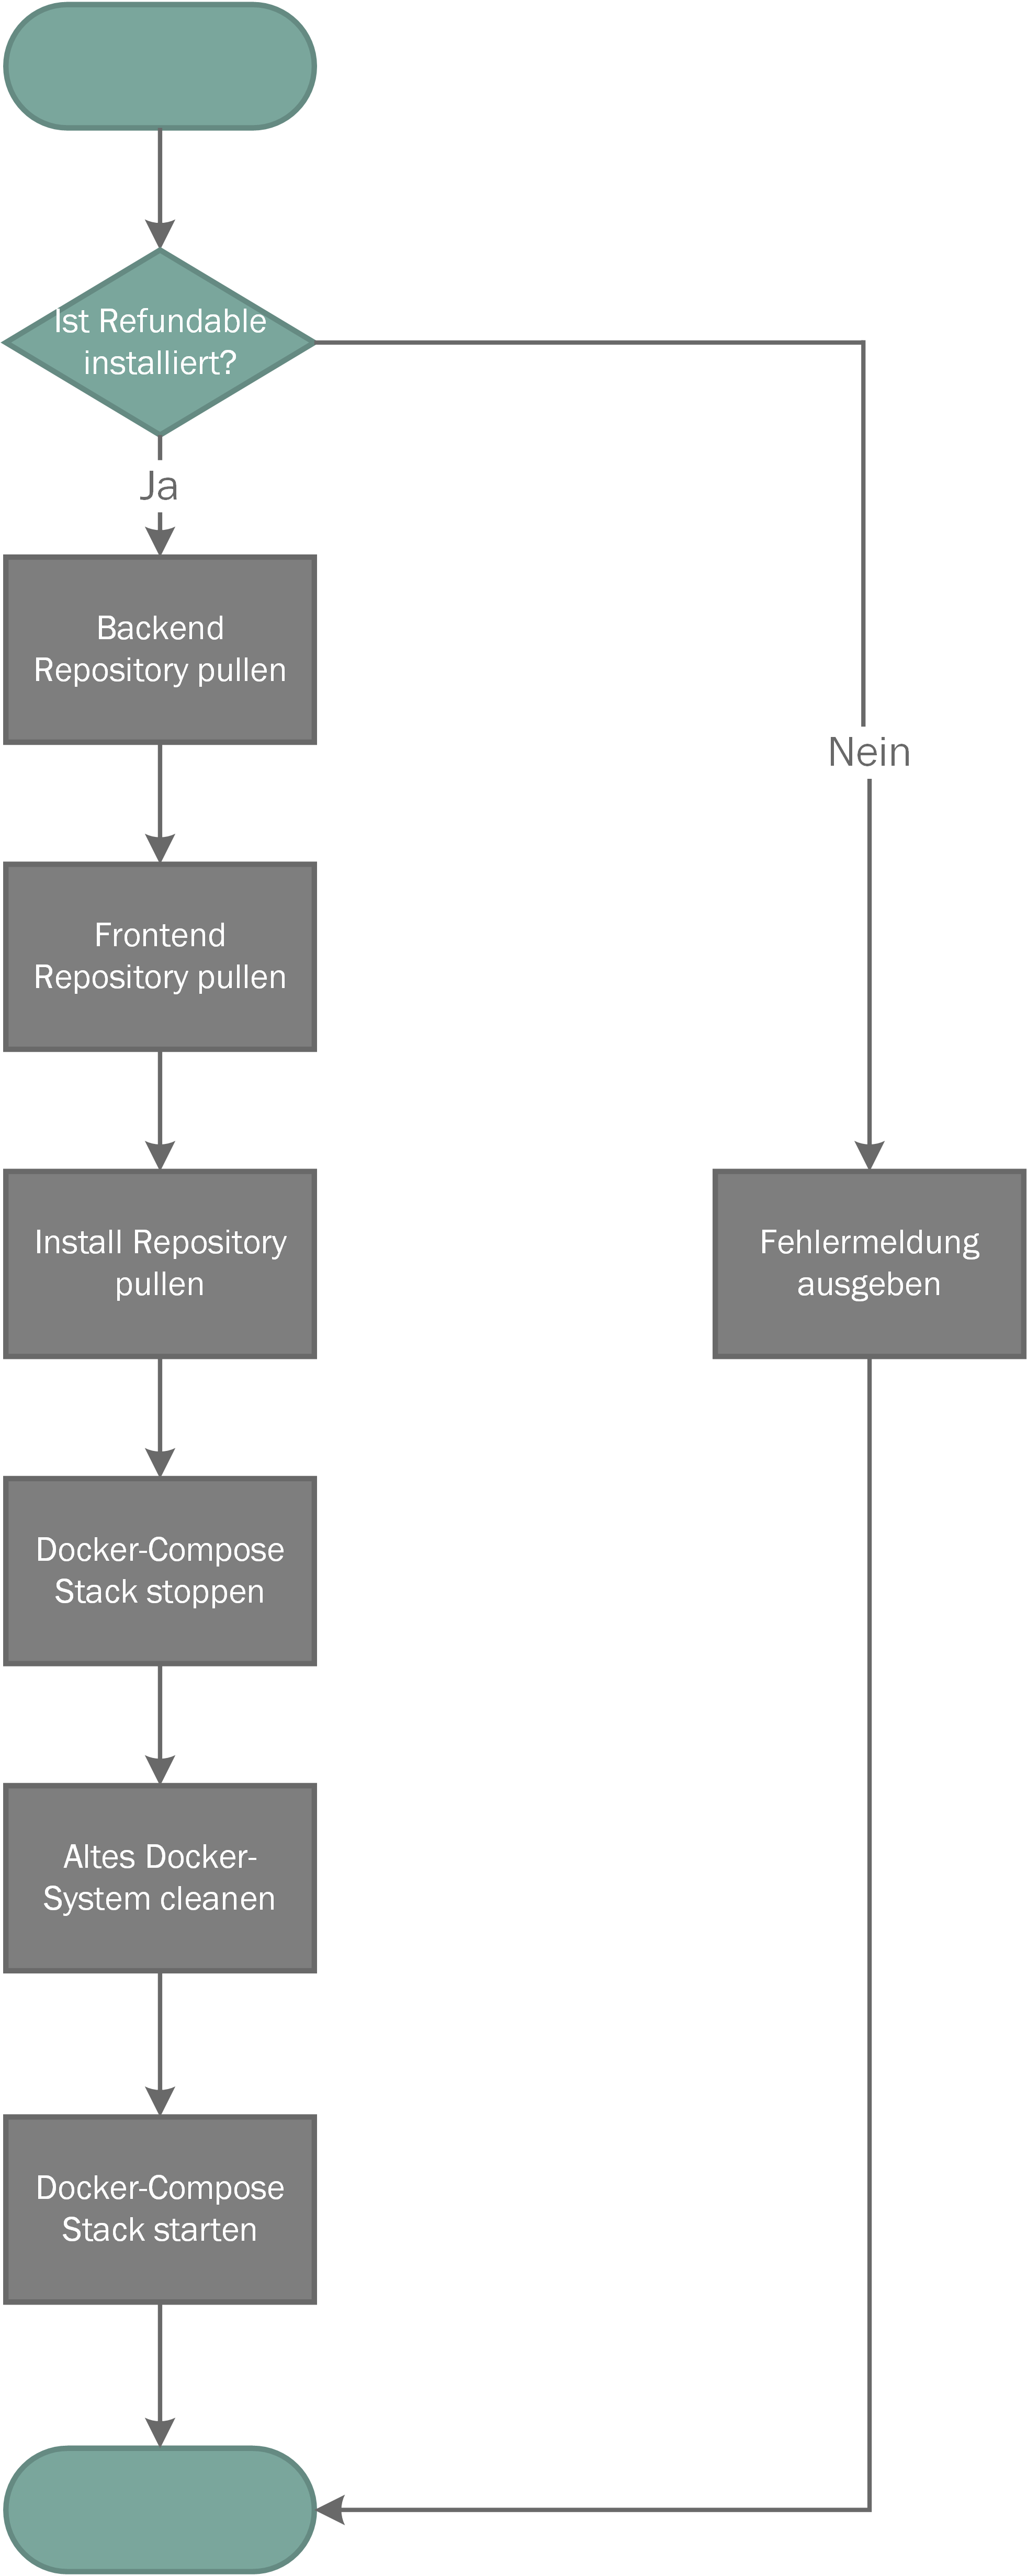
\includegraphics[width=0.47\linewidth]{images/mbeier_konzept/Update}
	\caption[Flussdiagramm über den Aktualisierungsvorgang]{Flussdiagramm über den Aktualisierungsvorgang}
	\label{fig:update}
\end{figure}
~\\
Der Aktualisierungsvorgang ist dem Installationsvorgang sehr ähnlich. Da es sich bei den installierten Dateien um solche aus Git-Repositories handelt, können diese auch einfach aktualisiert werden. Daraufhin wird nur noch ein Neustart des Systems durchgeführt.

\newpage

\textbf{Bereinigungsvorgang:}

\begin{figure}[H]
	\centering
	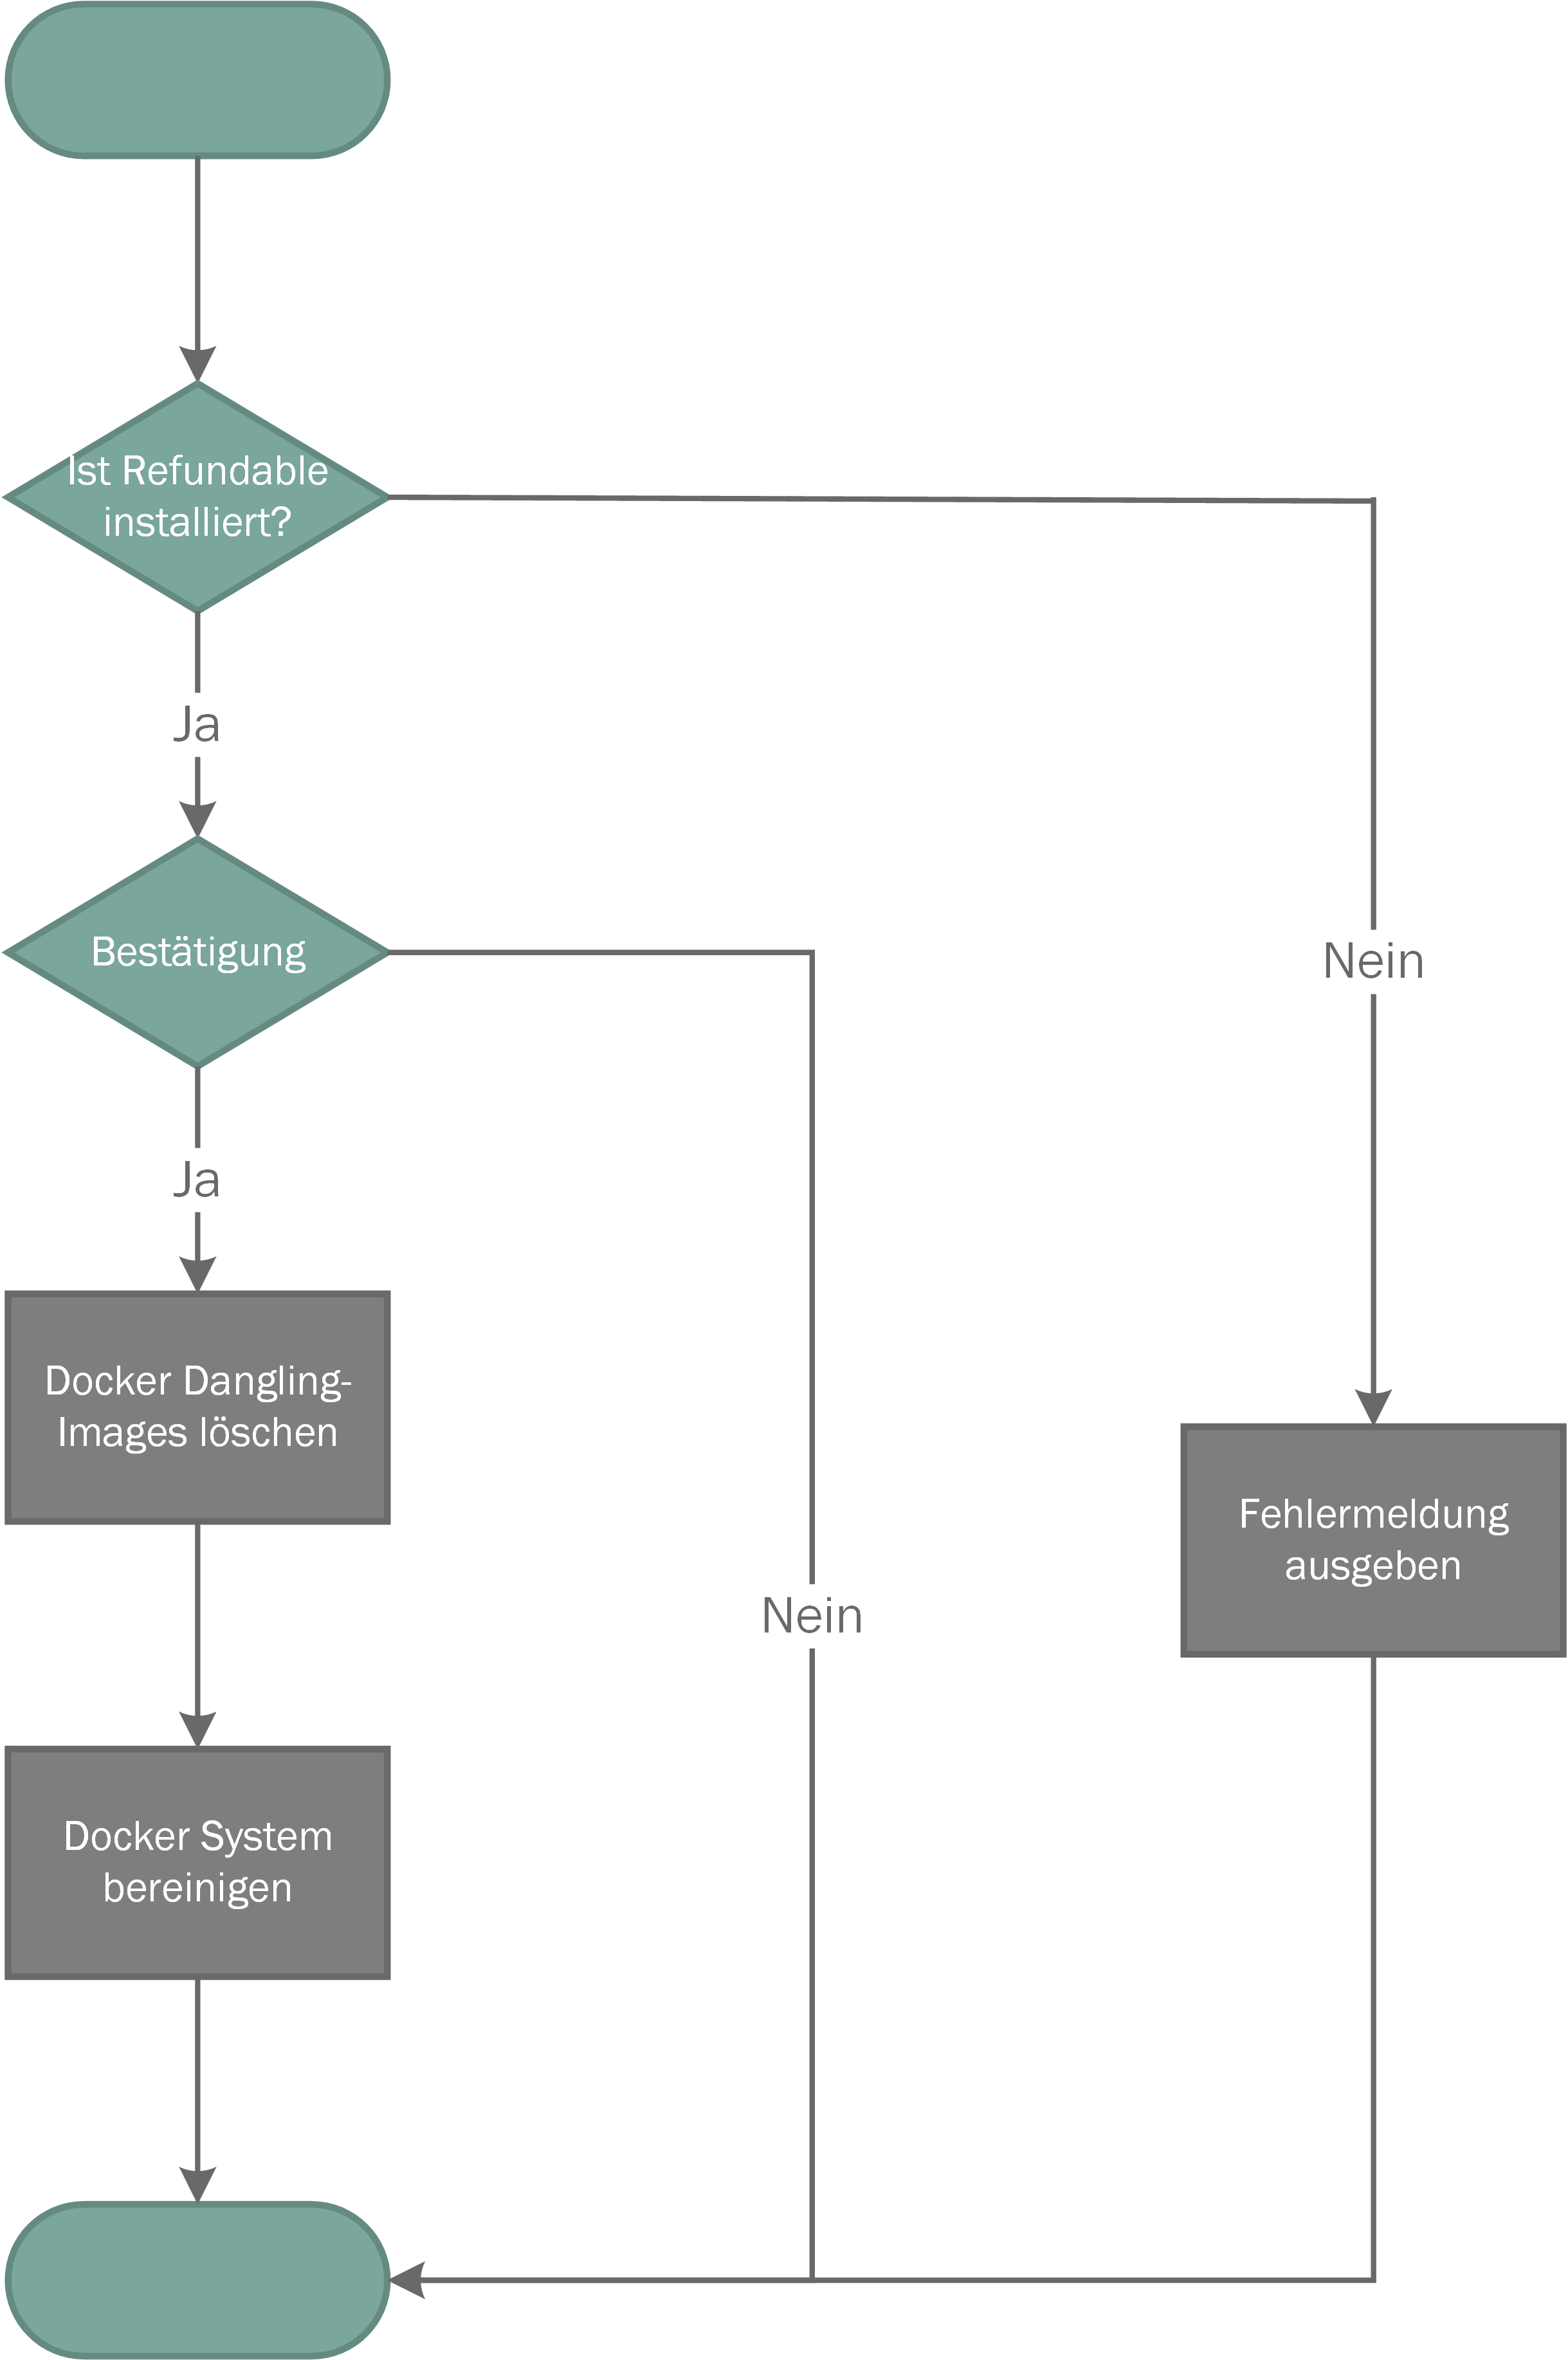
\includegraphics[width=0.55\linewidth]{images/mbeier_konzept/Clean}
	\caption[Flussdiagramm über den Bereinigungsvorgang]{Flussdiagramm über den Bereinigungsvorgang}
	\label{fig:clean}
\end{figure}
~\\
Der Bereinigungsvorgang nutzt die Docker Funktionen zum Löschen von nicht mehr benutzten Docker Images (Dangling Images). Nachdem werden die danach nicht mehr benutzten Ressourcen über die entsprechende Docker-Funktion aus dem System und der Docker Umgebung entfernt.

\newpage

\textbf{Deinstallation:}

\begin{figure}[H]
	\centering
	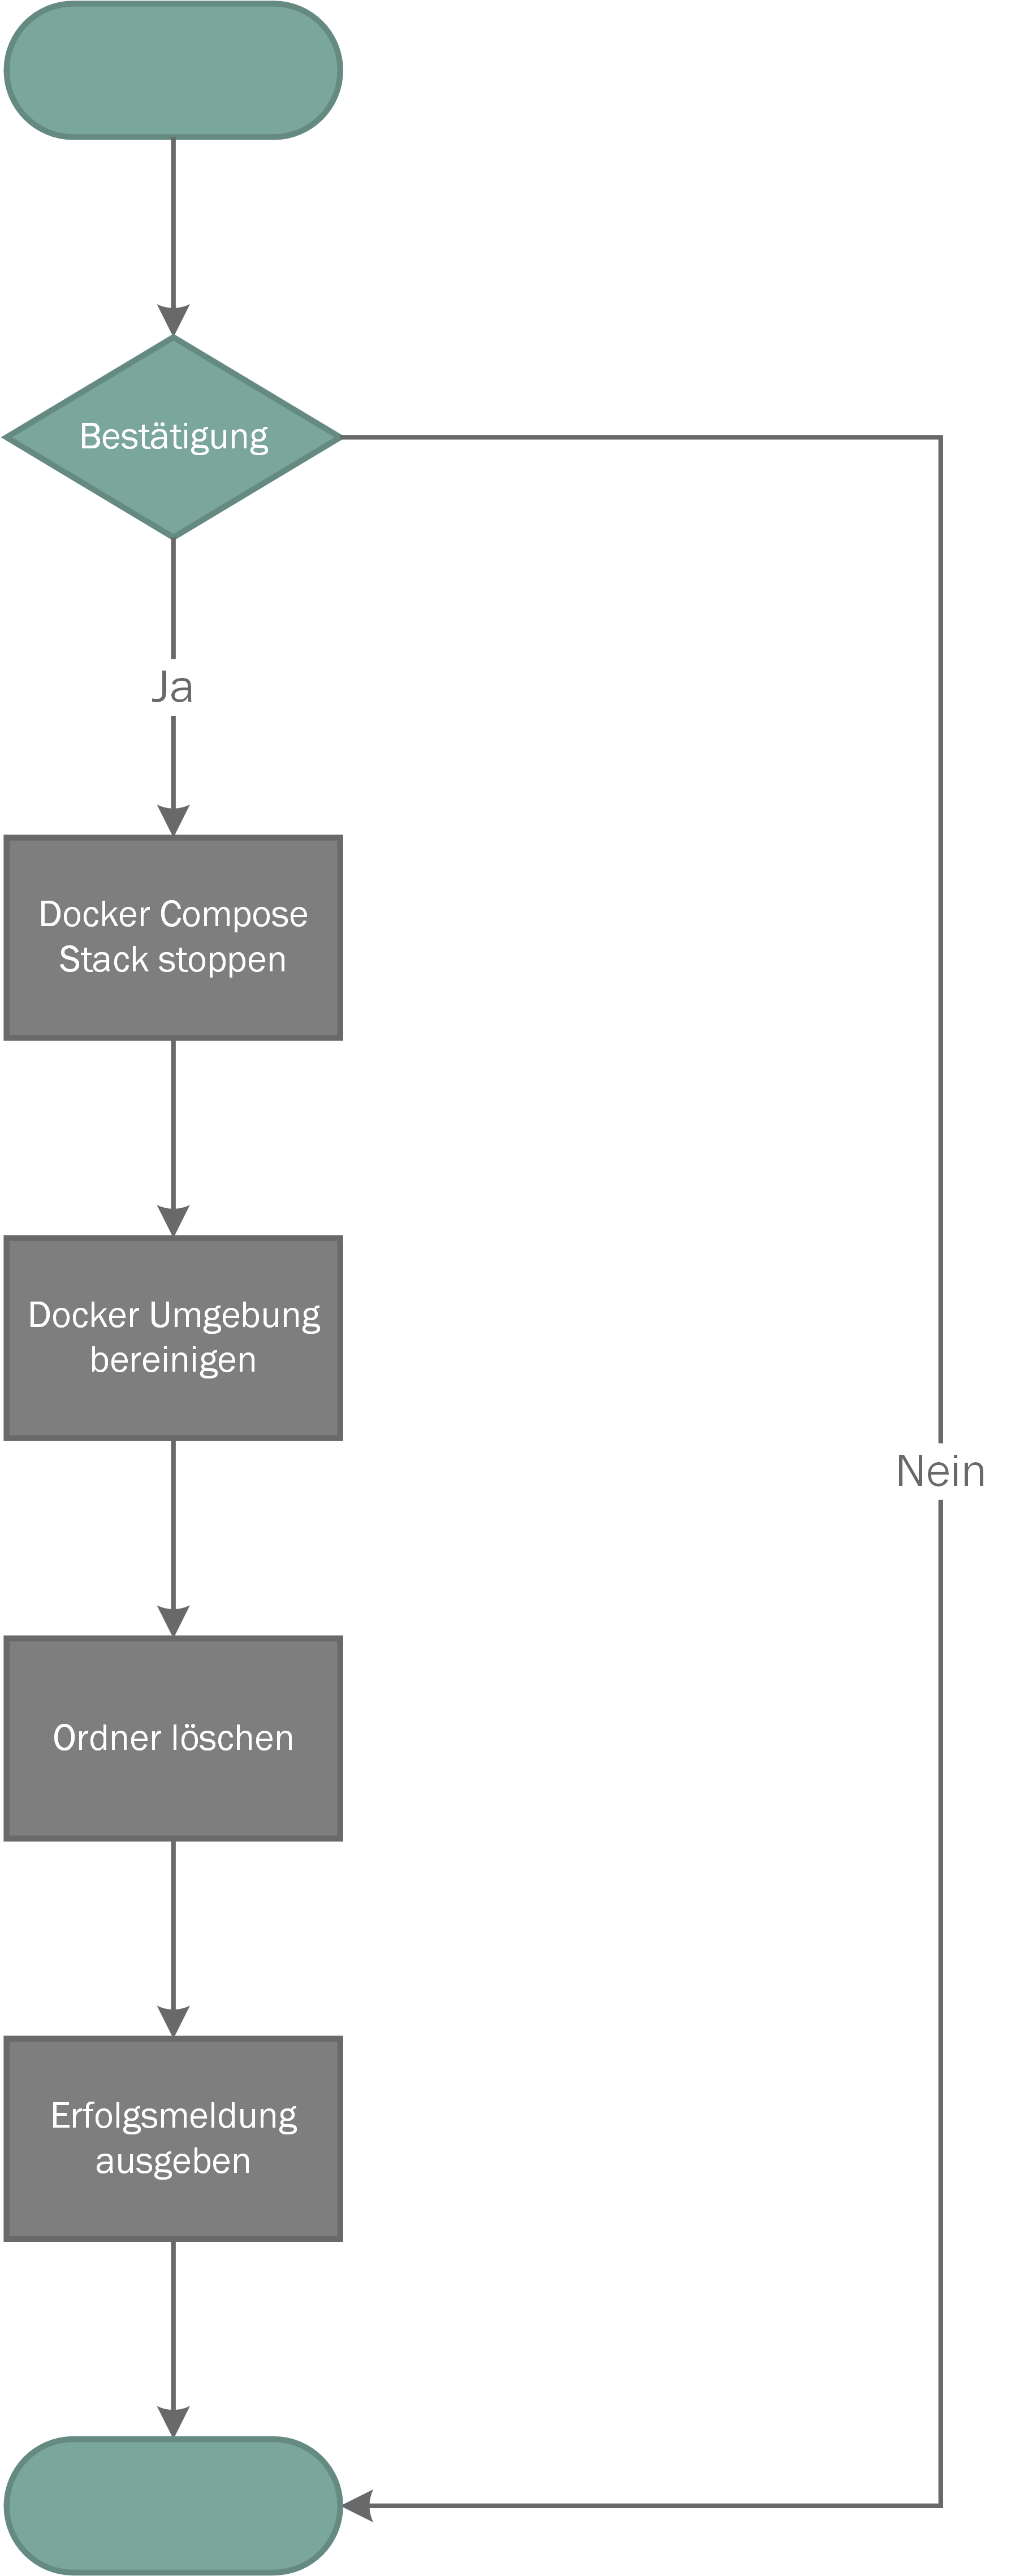
\includegraphics[width=0.48\linewidth]{images/mbeier_konzept/Purge}
	\caption[Flussdiagramm über die Deinstallation]{Flussdiagramm über die Deinstallation}
	\label{fig:purge}
\end{figure}
~\\
Der Vorgang hinter der Deinstallation löscht jegliche Information der Software aus der Docker Umgebung und auch alle Dateien, welche mit den Diensten assoziiert sind.

\newpage

\subsection{Datenmodell}

Auf Basis der zu erstellenden Anträge und der allgemeinen Nutzerverwaltung wurde folgendes Datenmodell entwickelt. Darin wurde speziell darauf geachtet, dass jegliche Information auch wirklich dort zu finden ist, wo sie auch auf einem papieren Antrag zu finden wäre. 

\begin{figure}[H]
	\centering
	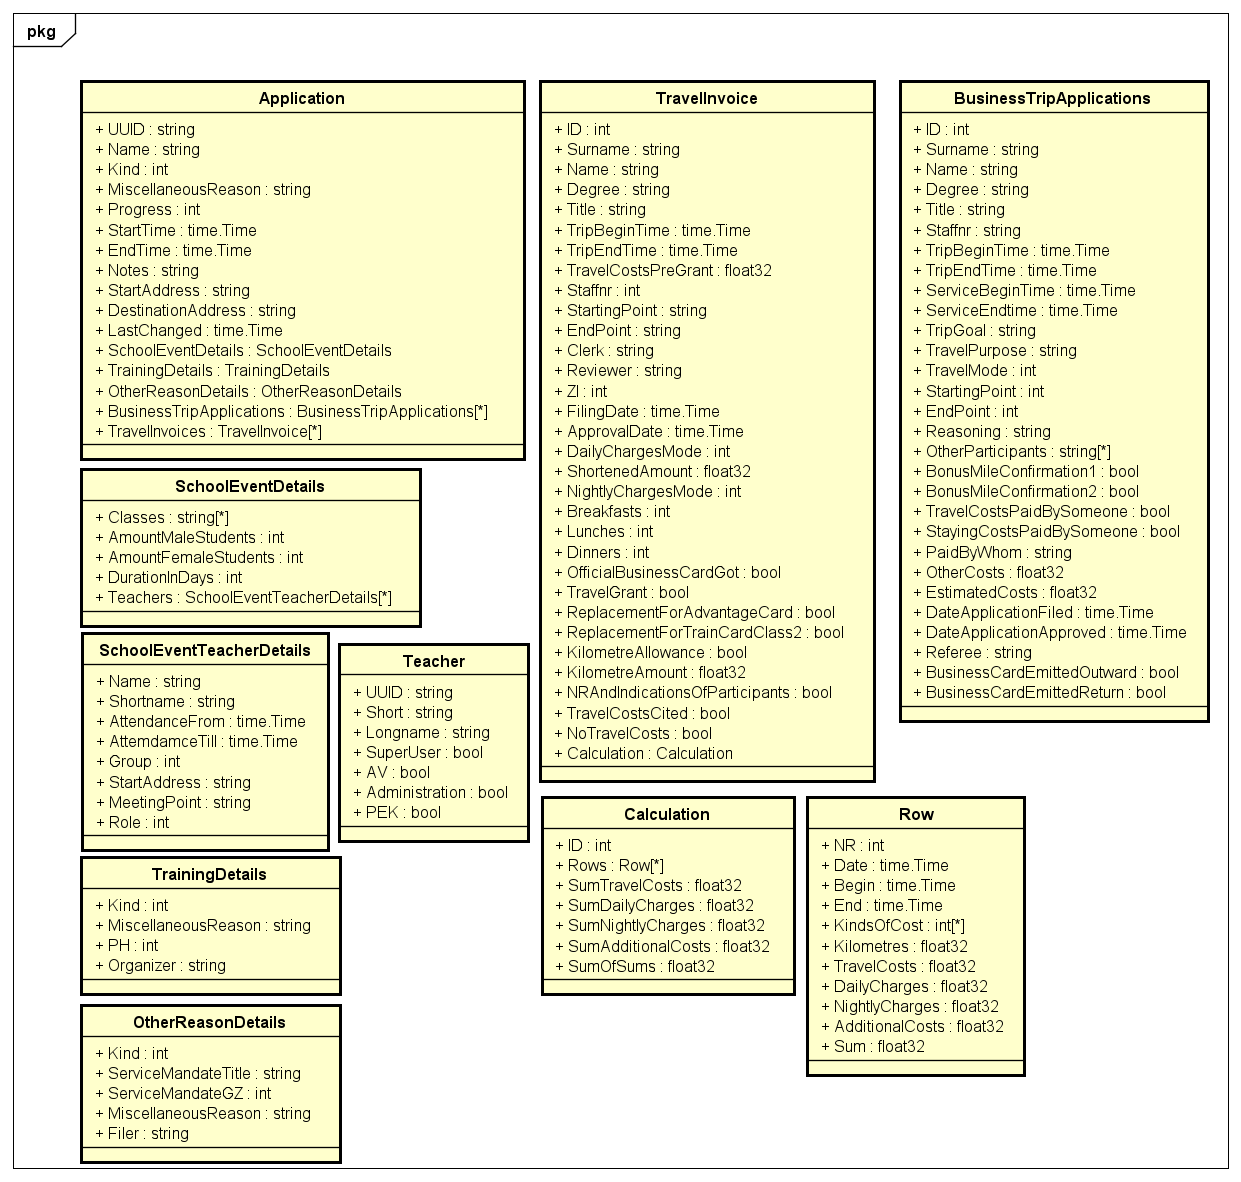
\includegraphics[width=\linewidth]{images/mbeier_konzept/Datamodel}
	\caption[Zentrales Datenmodell]{Das zentrale Datenmodell beinhaltet jegliche Daten, die von der Software benötigt werden.}
	\label{fig:datamodel}
\end{figure}

Im Gesamten gibt es zehn verschiedene Datenstrukturen, wobei hierbei neun die eigentlichen Anträge inklusive Subinformationen widerspiegeln und einer die Lehrkraft-Datenstruktur, welche das Schlüsselelement der Nutzerverwaltung darstellt.

\newpage

\subsection{REST-Schnittstelle}

Die REST-Schnittstelle im Backend ist die Kommunikationsschnittstelle mit dem Systemeigenen Frontend. Sie stellt jegliche Daten und generierte Files zur Verfügung und nimmt diverse Eingaben durch Lehrkräfte auf. Um jeweils diese Daten anzunehmen oder zurückzugeben werden sogenannte Endpoints erstellt. Diese sind in sich abgeschlossene Vorgänge, welche sich jeweils immer auf eine Aufgabe beschränken. Im folgenden Kapitel sind alle geplanten Endpoints beschrieben.

\subsubsection{Endpoints}
\label{chapter:endpoints}

Die folgende Tabelle beschreibt die geplanten Endpoints, wobei  sie jeweils mit der Protokollmethode (GET, POST, PUT oder DELETE), dem Pfad zum Endpoint, einer kurzen Beschreibung, Rückgaben, Eingaben und dem Erfordernis eines Tokens beschrieben werden.

\captionof{table}[REST-Endpoints 1]{Übersicht REST-Endpoints: Teil 1}
\label{table:endpoints1}
\begin{table}
	\centering
	\begin{tabular}{|l|l|l|l|l|}
		\hline
		\multicolumn{1}{|c|}{\textbf{Methode}} & \multicolumn{1}{c|}{\textbf{Endpoint}}                                                  & \multicolumn{1}{c|}{\textbf{Beschreibung}}                                                                  & \multicolumn{1}{c|}{\textbf{\begin{tabular}[c]{@{}c@{}}Rückgabe\\ (Erfolg)\end{tabular}}} & \multicolumn{1}{c|}{\textbf{Eingabe}}                                                                          \\ \hline
		
		
		POST                                   & /login                                                                                  & Loggt eine Lehrkraft ein                                                                                    & Tokenpaar                                                                                 & \begin{tabular}[c]{@{}l@{}}Benutzerinformationen\\ (Nutzername Passwort)\end{tabular}                          \\ \hline
		POST                                   & /logout                                                                                 & Loggt eine Lehrkraft aus                                                                                    & Erfolg                                                                                    & \multicolumn{1}{c|}{--}                                                                                        \\ \hline
		GET                                    & /login/refresh                                                                          & Erneuert einen Login                                                                                        & Tokenpaar                                                                                 & Refresh-Token (als Token)                                                                                      \\ \hline
		GET                                    & /getTeacherByShort                                                                      & \begin{tabular}[c]{@{}l@{}}Gibt Informationen zu \\ einer Lehrkraft zurück\end{tabular}                     & Lehrkraft                                                                                 & \begin{tabular}[c]{@{}l@{}}Abkürzung\\ einer  Lehrkraft\end{tabular}                                           \\ \hline
		GET                                    & /getTeacher                                                                             & \begin{tabular}[c]{@{}l@{}}Gibt Informationen zu\\ einer Lehrkraft zurück\end{tabular}                      & Lehrkraft                                                                                 & UUID einer Lehrkraft                                                                                           \\ \hline
		GET                                    & \begin{tabular}[c]{@{}l@{}}/setTeacher\\ Permissions\end{tabular}                       & \begin{tabular}[c]{@{}l@{}}Setzt die Berechtigungen\\ einer Lehrkraft\end{tabular}                          & Erfolg                                                                                    & \begin{tabular}[c]{@{}l@{}}Lehrkraft-\\ Berechtigungen\end{tabular}                                            \\ \hline
		GET                                    & \begin{tabular}[c]{@{}l@{}}/getActive\\ Applications\end{tabular}                       & \begin{tabular}[c]{@{}l@{}}Gibt alle aktiven Anträge\\ (einer Lehrkraft) zurück\end{tabular}                & \begin{tabular}[c]{@{}l@{}}Liste an\\ Anträgen\end{tabular}                               & \begin{tabular}[c]{@{}l@{}}optional: Name einer\\ Lehrkraft\end{tabular}                                       \\ \hline
		GET                                    & /getAllApplications                                                                     & Gibt alle Anträge zurück                                                                                    & \begin{tabular}[c]{@{}l@{}}Liste an\\ Anträgen\end{tabular}                               & \begin{tabular}[c]{@{}l@{}}optional: Name einer\\ Lehrkraft\end{tabular}                                       \\ \hline
		GET                                    & /getNews                                                                                & \begin{tabular}[c]{@{}l@{}}Gibt die letzt veränderten\\ Anträge zurück\end{tabular}                         & \begin{tabular}[c]{@{}l@{}}Liste an\\ Anträgen\end{tabular}                               & \multicolumn{1}{c|}{--}                                                                                        \\ \hline
		GET                                    & \begin{tabular}[c]{@{}l@{}}/getAdmin\\ Application\end{tabular}                         & \begin{tabular}[c]{@{}l@{}}Gibt alle Anträge zurück,\\ die von einem Admin \\ anzuschauen sind\end{tabular} & \begin{tabular}[c]{@{}l@{}}Liste an\\ Anträgen\end{tabular}                               & \multicolumn{1}{c|}{--}                                                                                        \\ \hline
		
	\end{tabular}
\end{table}	

\newpage
		
\captionof{table}[REST-Endpoints 2]{Übersicht REST-Endpoints: Teil 2}	
\label{table:endpoints2}
\begin{table}
	\centering
	\begin{tabular}{|l|l|l|l|l|}
		\hline
		\multicolumn{1}{|c|}{\textbf{Methode}} & \multicolumn{1}{c|}{\textbf{Endpoint}}                                                  & \multicolumn{1}{c|}{\textbf{Beschreibung}}                                                                  & \multicolumn{1}{c|}{\textbf{\begin{tabular}[c]{@{}c@{}}Rückgabe\\ (Erfolg)\end{tabular}}} & \multicolumn{1}{c|}{\textbf{Eingabe}}                                                                          \\ \hline
		
		GET                                    & /getApplication                                                                         & \begin{tabular}[c]{@{}l@{}}Gibt Informationen zu\\ einem Antrag zurück\end{tabular}                         & Antrag                                                                                    & UUID des Antrages                                                                                              \\ \hline
		POST                                   & /createApplication                                                                      & Erstellt einen Antrag                                                                                       & Erfolg                                                                                    & Antragsdaten                                                                                                   \\ \hline
		PUT                                    & /updateApplication                                                                      & Aktualisiert einen Antrag                                                                                   & Erfolg                                                                                    & Antragsdaten                                                                                                   \\ \hline
		DELETE                                 & /deleteApplication                                                                      & Löscht einen Antrag                                                                                         & Erfolg                                                                                    & Antragsdaten                                                                                                   \\ \hline
		GET                                    & \begin{tabular}[c]{@{}l@{}}/getAbsenceForm\\ ForClasses\end{tabular}                    & \begin{tabular}[c]{@{}l@{}}Erstellt das Abwesenheits-\\ formular von Klassen\end{tabular}                   & PDF                                                                                       & \begin{tabular}[c]{@{}l@{}}UUID des Antrages, \\ optional: Liste an Klassen\end{tabular}                       \\ \hline
		GET                                    & \begin{tabular}[c]{@{}l@{}}/getAbsenceForm\\ ForTeacher\end{tabular}                    & \begin{tabular}[c]{@{}l@{}}Erstellt das Abwesenheits-\\ formular einer Lehrkraft\end{tabular}               & PDF                                                                                       & \begin{tabular}[c]{@{}l@{}}UUID des Antrages, \\ Name der Lehrkraft\end{tabular}                               \\ \hline
		GET                                    & \begin{tabular}[c]{@{}l@{}}/getCompensation\\ ForEducational\\ SupportForm\end{tabular} & \begin{tabular}[c]{@{}l@{}}Erstellt das Formular\\ für pädagogische Betreuung\end{tabular}                  & PDF                                                                                       & UUID des Antrages                                                                                              \\ \hline
		GET                                    & \begin{tabular}[c]{@{}l@{}}/getTravel\\ InvoiceForm\end{tabular}                        & \begin{tabular}[c]{@{}l@{}}Erstellt ein \\ Reiserechnungsformular\end{tabular}                              & PDF                                                                                       & \begin{tabular}[c]{@{}l@{}}UUID des Antrages, \\ Name der Lehrkraft, \\ ID der Reiserechnung\end{tabular}      \\ \hline
		GET                                    & \begin{tabular}[c]{@{}l@{}}/getBusinessTrip\\ ApplicationForm\end{tabular}              & \begin{tabular}[c]{@{}l@{}}Erstellt ein \\ Dienstantragsformular\end{tabular}                               & PDF                                                                                       & \begin{tabular}[c]{@{}l@{}}UUID des Antrages, \\ Name der Lehrkraft, \\ ID des Dienstreiseantrags\end{tabular} \\ \hline
		GET                                    & \begin{tabular}[c]{@{}l@{}}/getTravel\\ InvoiceExcel\end{tabular}                       & \begin{tabular}[c]{@{}l@{}}Erstellt eine Reiserechnung\\ als Excel-Datei\end{tabular}                       & Excel                                                                                     & \begin{tabular}[c]{@{}l@{}}UUID des Antrages, \\ Name der Lehrkraft, \\ ID der Reiserechnung\end{tabular}      \\ \hline
		GET                                    & \begin{tabular}[c]{@{}l@{}}/getBusinessTrip\\ ApplicationExcel\end{tabular}             & \begin{tabular}[c]{@{}l@{}}Erstellt einen Dienstantrag\\ als Excel-Datei\end{tabular}                       & Excel                                                                                     & \begin{tabular}[c]{@{}l@{}}UUID des Antrages, \\ Name der Lehrkraft, \\ ID des Dienstreiseantrags\end{tabular} \\ \hline
		POST                                   & /saveBillingReceipt                                                                     & \begin{tabular}[c]{@{}l@{}}Speichert einen \\ Beleg als PDF ab\end{tabular}                                 & \multicolumn{1}{c|}{--}                                                                   & PDF                                                                                                            \\ \hline
	\end{tabular}
\end{table}

\newpage

\subsubsection{Token System}

Die Implementierung eines nicht-persistenten Token Systems, um die Kommunikation mit der REST-Schnittstelle weiter zu schützen, ist gerade, wenn es sich um sensible Daten handelt sehr wichtig. Ansonsten könnte jeder einfach die Endpoints der Schnittstelle ansprechen. Durch die Ausgabe von sogenannten \enquote{Access Tokens} und \enquote{Refresh Tokens} werden diese jedoch abgesichert. Dies geschieht dadurch, dass diese bei jeder Anfrage nach dem Login mit übergeben werden müssen (im Headerfeld \enquote{Authorization}), wodurch sich der Absender als eingeloggte Lehrkraft verifiziert. Anfragen ohne Tokens werden in Folge automatisch abgewiesen. 
\\Diese Tokens sind verschlüsselte Zeichenketten, welche nur durch das Backend entschlüsselbar sind, da nur das System selbst den Schlüssel hierfür kennt. Im Token selbst werden Informationen über die Sitzung und den Nutzer gespeichert, sodass er nur durch die Angabe des Tokens verifiziert werden kann.\\
Das \enquote{Access Token} ist genau 15 Minuten lang gültig und erlaubt solange direkten Zugriff auf die Schnittstelle. Sobald dieses abgelaufen ist, kann mit dem \enquote{Refresh Token}, welches 7 Tage lang gültig ist, ein neues Tokenpaar bei der Schnittstelle generiert werden. Da es sich um zwei komplett neue Tokens handelt, verlängert sich auch die Gültigkeit des Logins hierbei. Sollte keines der beiden Token mehr gültig sein, so muss ein neues Paar durch einen neuen Loginvorgang erstellt werden.

\subsection{Backend}
Um jene in  \autoref{chapter:endpoints} beschriebenen Endpoints auch mit Funktionalität ausstatten zu können, müssen entsprechende Methoden im Backend implementiert werden. Hierzu gehören hauptsächlich die Schnittstellen zu folgenden Diensten und die Implementierungen von Hauptfunktionen des Systems. Diese sind in den folgenden Abschnitten beschrieben.

\subsubsection{Untis}

Die offizielle Untis-Schnittstelle ermöglicht dem System die Abfrage des aktuellen Stunden- und Supplierplans. Dadurch können diese Informationen auch auf den etwaigen Formularen direkt genutzt werden. Um mit dieser Schnittstelle einfach kommunizieren zu können, ist folgender Aufbau und Implementierung eines REST-Clients im Backend geplant. Mit Hilfe diesen kann das System einfach die Sitzung, welche schon durch die REST-Schnittstelle existiert, weiter nutzen und somit möglichst effizient arbeiten.

\begin{figure}[H]
	\centering
	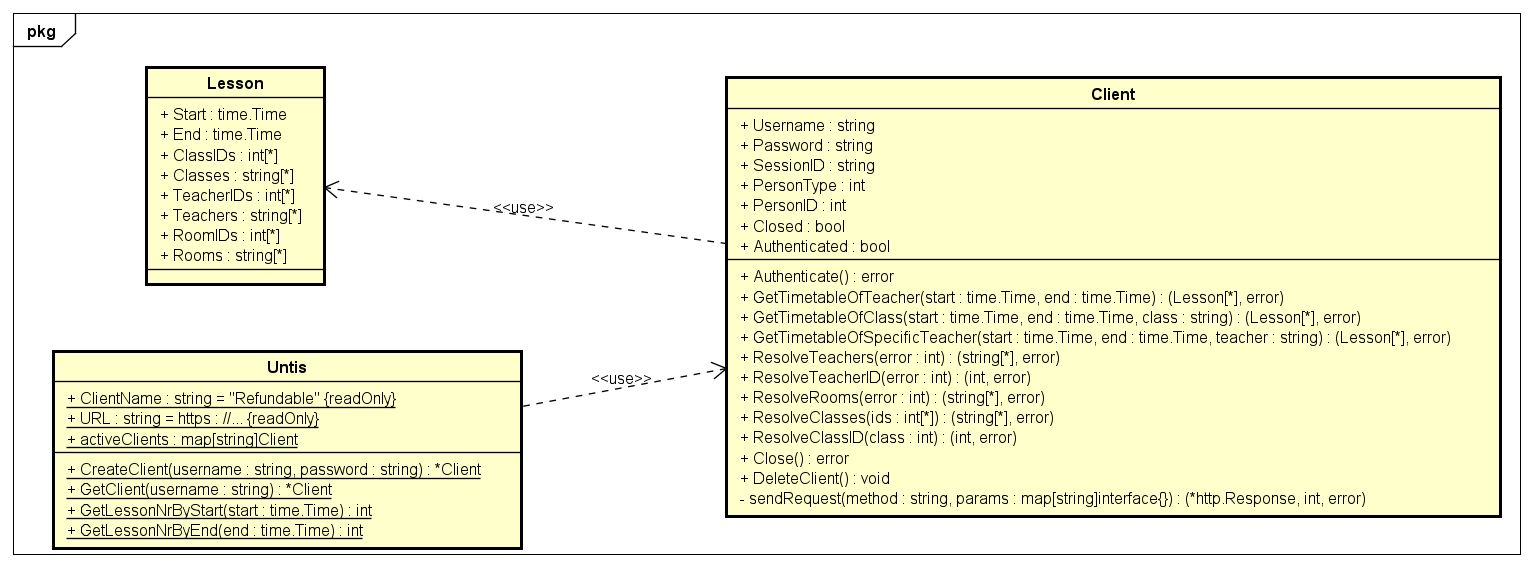
\includegraphics[width=\linewidth]{images/mbeier_konzept/Untis}
	\caption[Untis API-Client UML-Klassendiagramm]{UML-Klassendiagramm des Untis API-Client für das Abfragen von Stundenplaninformationen.}
	\label{fig:untis}
\end{figure}

\newpage

\subsubsection{LDAP}

LDAP ist ein Zugriffsprotokoll um auf ein Active Directory zugreifen zu können. In diesem wird im tgm weitere Informationen zu den Lehrkräften und Schülern gespeichert. Um diese Daten einsehen zu können, muss man sich bei diesem Dienst anmelden, was mit den jeweils eigenen tgm-Account Zugangsdaten möglich ist. Dadurch ist die Anmeldung mit den tgm-Nutzerdaten zu realisieren. Des Weiteren ist die Abfrage weiterer benötigter Daten hierdurch möglich. Der Ablauf einer solchen Interaktion über LDAP wird in folgendem Flussdiagramm veranschaulicht.

\begin{figure}[H]
	\centering
	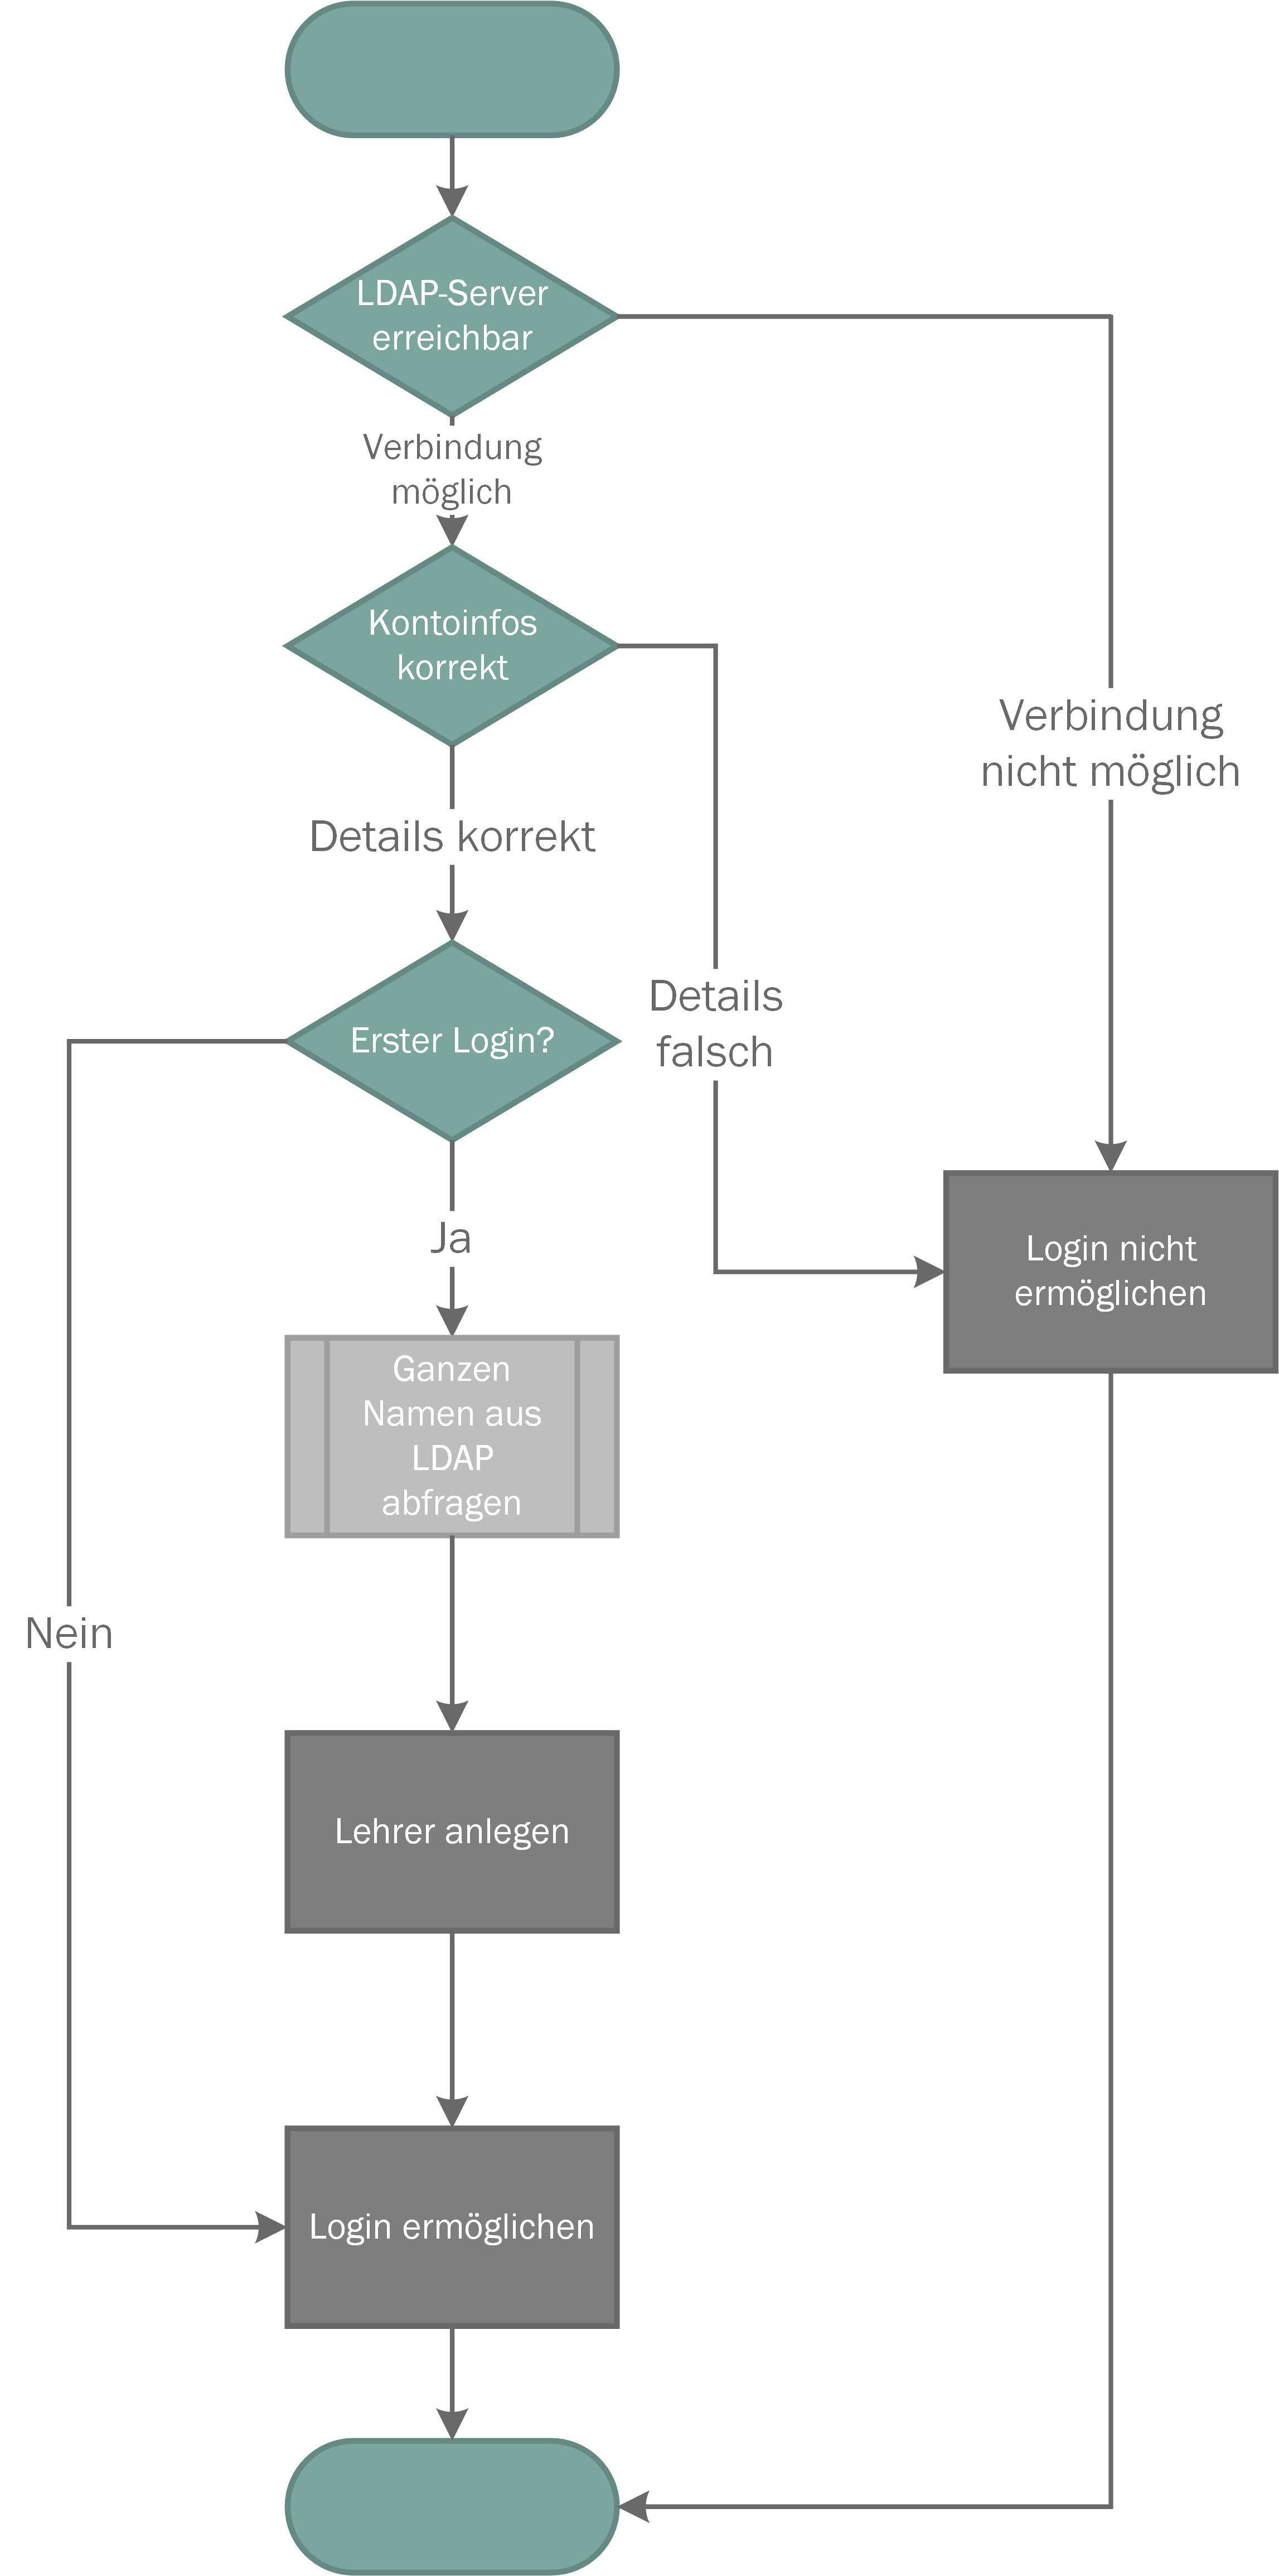
\includegraphics[width=0.5\linewidth]{images/mbeier_konzept/LDAP_Authenticate}
	\caption[Authentifizierung über LDAP]{Authentifizierung über den tgm-eigenen LDAP Server}
	\label{fig:ldapauthenticate}
\end{figure}

\newpage

Um jenen in \autoref{fig:ldapauthenticate} abgebildeten Ablauf einfach implementieren zu können, bietet sich folgender Aufbau eines LDAP-Clients an. Dieser kann dann hierbei die Zugangsdaten durch eine einfache Anmeldung beim Dienst verifizieren und auch die benötigten Daten, den kompletten Namen der Lehrkraft, beim Dienst abfragen.

\begin{figure}[H]
	\centering
	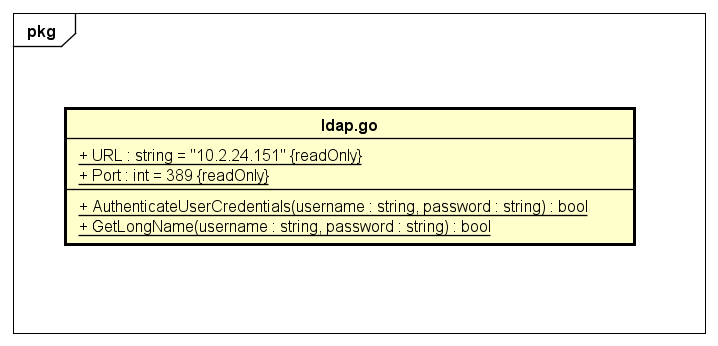
\includegraphics[width=\linewidth]{images/mbeier_konzept/LDAP}
	\caption[lLDAP UML-Klassendiagramm]{UML-Klassendiagramm des LDAP Packages für die Authentifizierung von Lehrkräften}
	\label{fig:ldap}
\end{figure}

\newpage

\subsubsection{Dateierstellung}

Die Datei- und Formularerstellung ist die Hauptfunktion der Software. Das Generieren folgender Forms wird unterstützt. Bei \enquote{Reiserechnung} und \enquote{Dienstreiseantrag} werden auf Grund des festgelegten Designs auch eine Excel Variante angeboten, in der dieses umgesetzt ist. Das Format steht hierbei für Hoch- oder Querformat, wobei Portrait das Hochformat und Landscape das Querformat ist.

\captionof{table}[Dateierstellung - Dateien]{Übersicht über die verschiedenen Dateien, die durch das Backend erstellt werden.}	
\label{tbl:files}
\begin{table}
	\centering
	\begin{tabular}{|l|l|l|}
		\hline
		\multicolumn{1}{|c|}{\textbf{Formular}} & \multicolumn{1}{c|}{\textbf{Dateityp}} & \multicolumn{1}{c|}{\textbf{Format}} \\ \hline
		Abwesenheitsmeldung eines Jahrganges & PDF & Portrait \\ \hline
		Abwesenheitsmeldung eines Lehrers & PDF & Portrait \\ \hline
		Abgeltung für pädagogische Betreuung & PDF & Portrait \\ \hline
		Reiserechnung & PDF & Landscape \\ \hline
		Dienstreiseantrag & PDF & Portrait \\ \hline
		Reiserechnung & Excel & Landscape \\ \hline
		Dienstreiseantrag & Excel & Portrait \\ \hline
	\end{tabular}
\end{table}

~\\
Alle eigens generierten PDFs sind jedenfalls mit einer Kopfzeile ausgestattet. In dieser ist in der linken Ecke das tgm-Logo zu sehen, in der Mitte steht der Name des Formulars (siehe \autoref{tbl:files}) und rechts ein QR-Code, welcher einen nach dem Scan auf die Website führt und den zugehörigen Antrag dort direkt öffnet.

\begin{figure}[H]
	\centering
	
\includegraphics[width=\linewidth]{images/mbeier_konzept/Kopfleiste_PDF_border}
	\caption[Kopfleiste PDF-Datei]{Beispiel einer Kopfleiste in den vom Backend generierten PDF-Dateien}
	\label{fig:kopfleiste-pdf}
\end{figure}

